% % !TEX root = ../main.tex

% % Indicate the main file. Must go at the beginning of the file.

% %---------------------------------------------------------------------
% % CHAPTER TEMPLATE
% %---------------------------------------------------------------------
% %[
% % \chapter{Methode} % Main chapter title
% \label{Methode} % Change X to a consecutive number; for referencing this chapter elsewhere, use \ref{ChapterX}

% %--------------------------------------------------------------------------------
% % SECTION Stand von Konkurenzprodukten
% %--------------------------------------------------------------------------------

% \section{Recherche bestehende Produkte}

% \begin{table}[h!]
%     \centering
%     \begin{tabular}{|>{\raggedright\arraybackslash}p{3cm}|>{\raggedright\arraybackslash}p{3cm}|>{\raggedright\arraybackslash}p{3cm}|>{\raggedright\arraybackslash}p{3cm}|>{\raggedright\arraybackslash}p{3cm}|}
%         \hline
%         \textbf{Name} & \textbf{AMiT MVB Analyzer} & \textbf{Ci4Rail MIO03 MVB/CAN Sniffer} & \textbf{Yacer MVB-Analyzer Protocol Analyzer} \\
%         \hline
%         \textbf{Interface Typen} & EMD / ESD & & \\
%         \hline
%         \textbf{Galvanische Trennung} & Ja & & \\
%         \hline
%         \textbf{Connectors} & 2 × D-Sub DE-9, RJ45,  & & \\
%         \hline
%         \textbf{Communication Rate MVB} & 1.5 Mbps ±0.01 \% & & \\
%         \hline
%         \textbf{Communication Rate Endgerät} & ETH: 10 / 100 Mbps & & \\
%         \hline
%         \textbf{Spannungs-versorgung} & 16,8 V - 33,6 V DC & & \\
%         \hline
%         \textbf{Gewicht} & 0,9 kg & & \\
%         \hline
%         \textbf{Dimensionen (b × h × l)} & (33 × 228 × 87) mm & & \\
%         \hline
%         \textbf{Analyse Tool} & WireShark & & \\
%         \hline
%     \end{tabular}
%     \caption{Vergleich MVB Sniffer}
%     \label{tab:mvb_analyzer}
% \end{table}

% %-----------------------------------
% % SUBSECTION "Amit"
% %-----------------------------------
 
% \subsection{Konkurenz 1 (Amit Transportation)}
% \textcolor{red}{Amit MVB Analyzer}

% \begin{figure}[H]
%     \centering
%     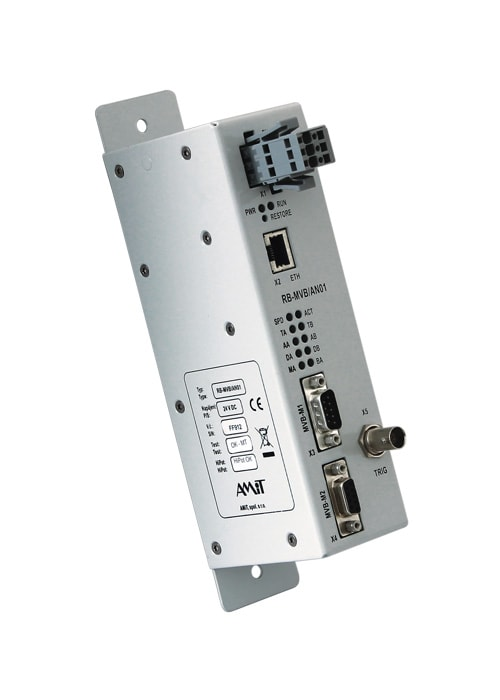
\includegraphics[width=0.5\linewidth]{Figures/Chap3/Konkurenz/Amit.jpg}
%     \caption{Bild von Herstellerseite}
%     \label{fig:enter-label}
% \end{figure}

% %-----------------------------------
% % SUBSECTION "Ci4Rail"
% %-----------------------------------

% \subsection{Konkurenz 2 (Ci4Rail)}
% \textcolor{red}{IP\ Based\ Sniffer}

% \begin{figure}[H]
%     \centering
%     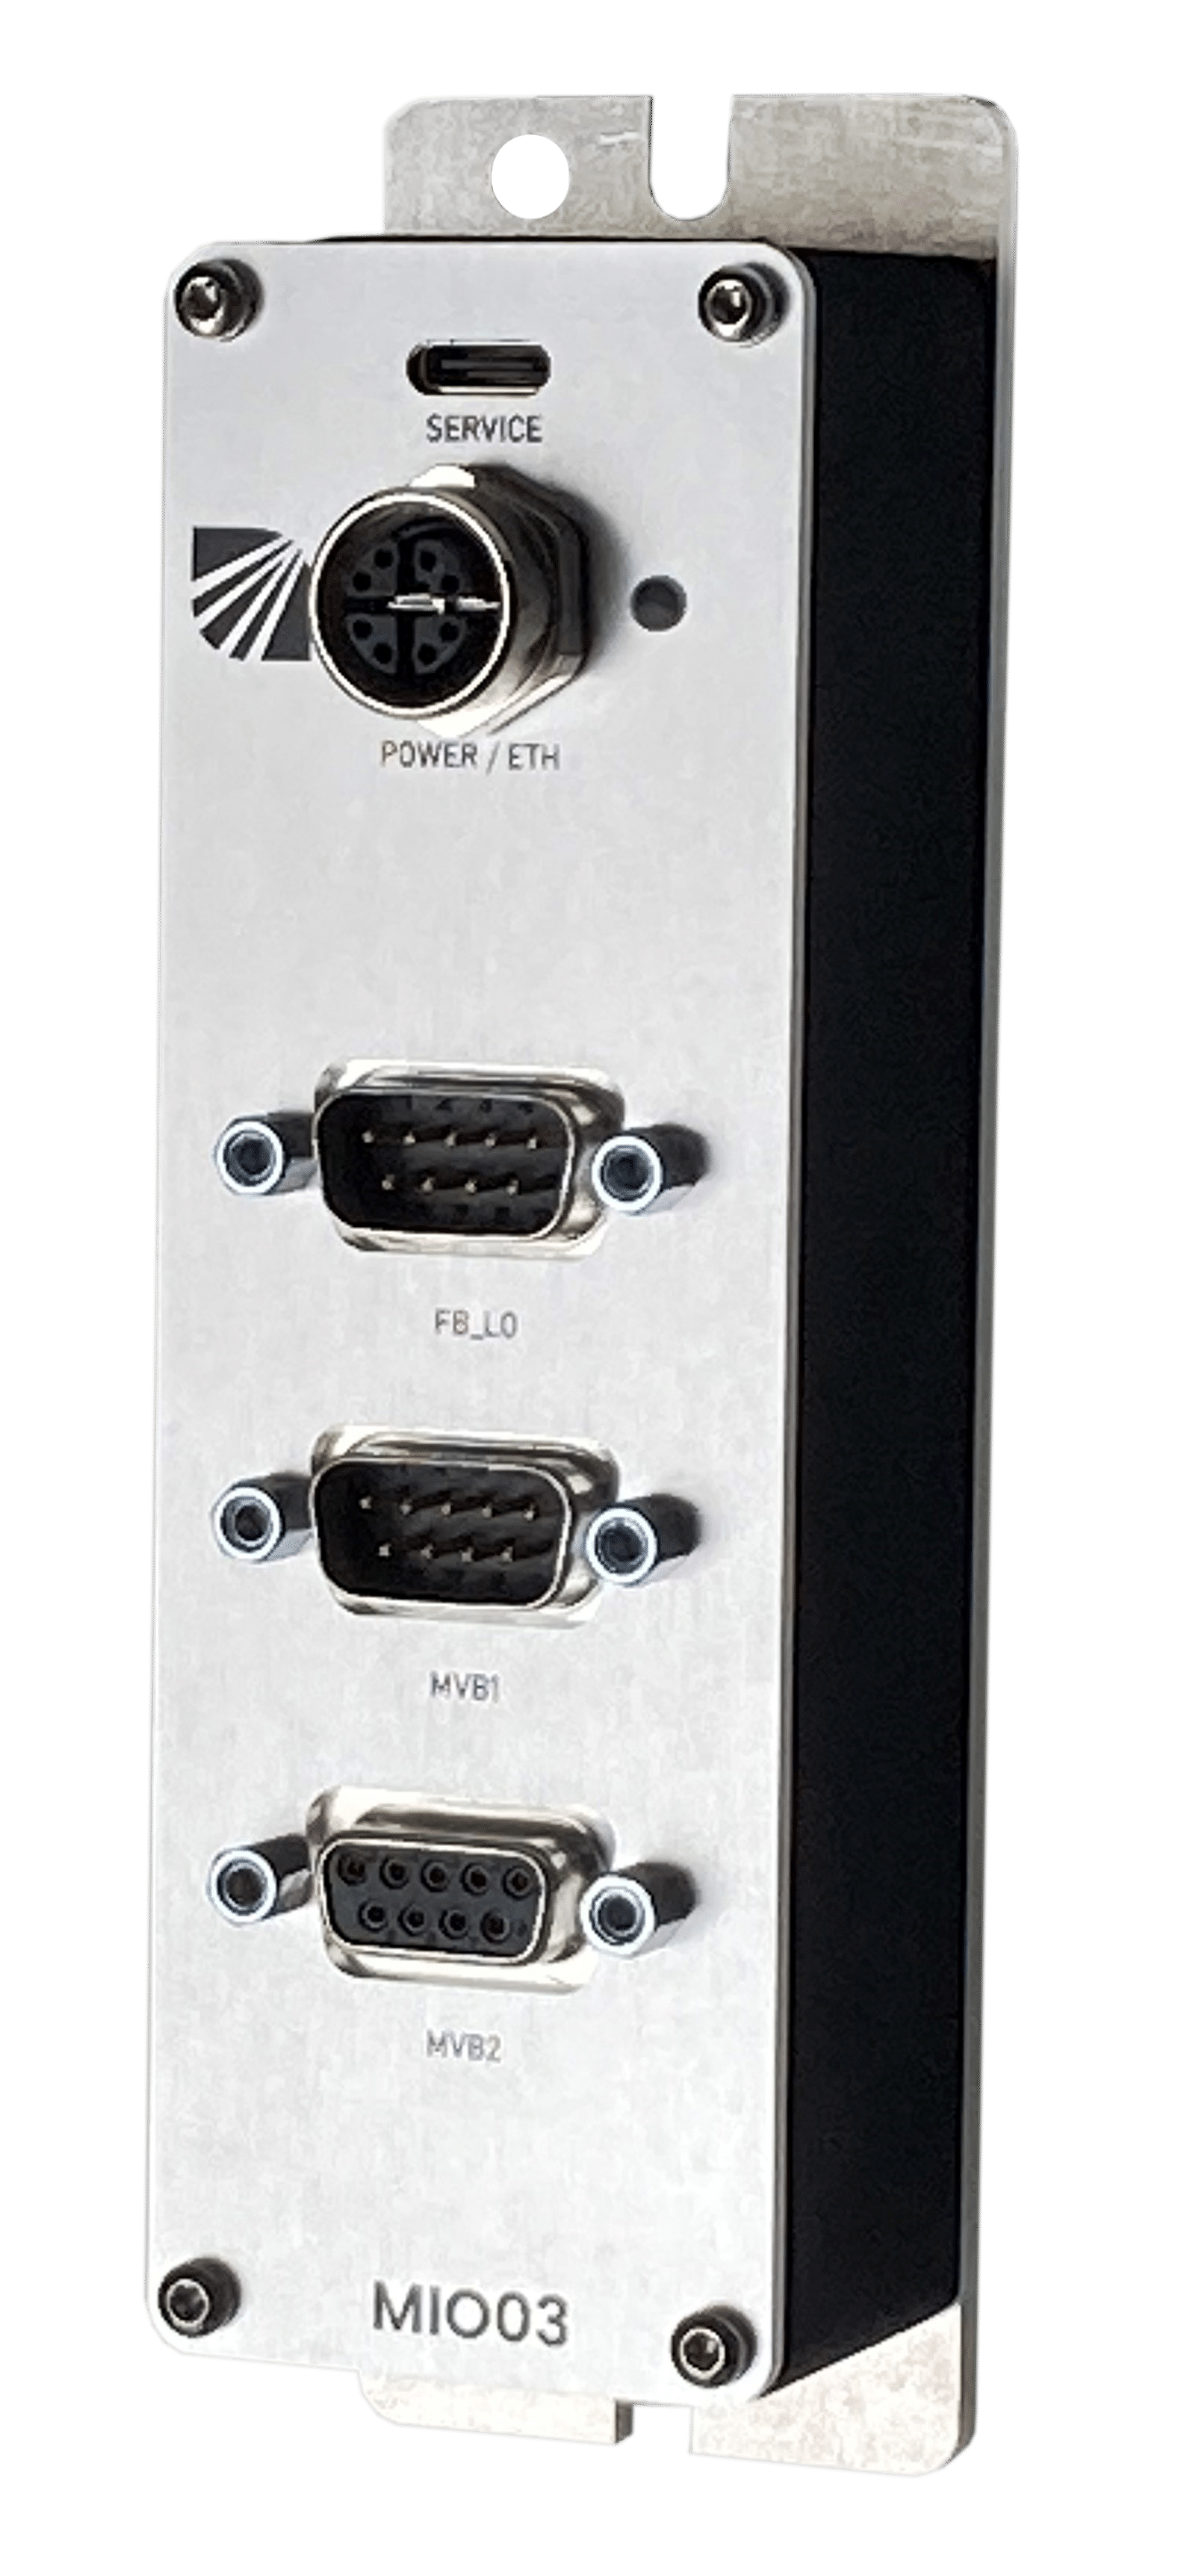
\includegraphics[width=0.5\linewidth]{Figures/Chap3/Konkurenz/CI4Rail.png}
%     \caption{Bild von Herstellerseite}
%     \label{fig:enter-label}
% \end{figure}


% %-----------------------------------
% % SUBSECTION "Yacer"
% %-----------------------------------

% \subsection{Konkurenz 3 (Yacer MVB-Analyzer Protocol Analyzer)}
% \textcolor{red}{Ebenfalls IP Based}

% \begin{figure}[H]
%     \centering
%     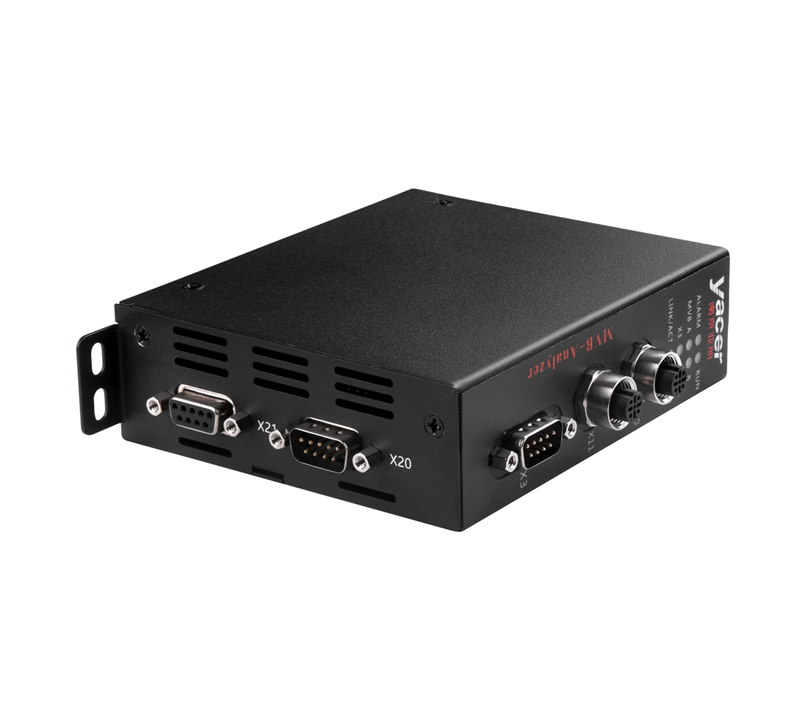
\includegraphics[width=0.5\linewidth]{Figures/Chap3/Konkurenz/Yacer.jpg}
%     \caption{Bild von Herstellerseite}
%     \label{fig:enter-label}
% \end{figure}


% %-----------------------------------
% % SUBSECTION "Abgrenzung"
% %-----------------------------------

% \subsection{Angrenzung zu den bestehenden Produkten}
% \textcolor{red}{Was macht unser Sniffer anders/ besser}]

% %---------------------------------------------------------------------
% % SECTION Busauslastung messen
% %---------------------------------------------------------------------

% \section{Busauslastung messen}
% Um zu beurteilen, ob Bluetooth Low Energy (BLE) eine geeignete Lösung für die Übertragung von Telegrammen vom Sniffer zum Endgerät darstellt, wurde ein Versuch unternommen, die Busauslastung mittels Oszilloskop zu analysieren. Ziel war es, abzuschätzen, ob die dabei gewonnenen effektiven Nutzdaten über BLE übertragen werden können. Gleichzeitig sollte geprüft werden, ob eine direkte Übertragung aller Rohdaten möglich ist oder ob eine Filterung der Telegramme erforderlich wäre.

% Für die Analyse wurden zwei Messungen durchgeführt: Eine unter Normallast und eine unter Volllast. Die Volllast wurde simuliert, indem der Depot-Diagnosespeicher auf dem Fahrzeugdisplay abgerufen wurde. Dies führte dazu, dass der Speicher die entsprechenden Daten über den Bus an das Display sendete, was kurzfristig zu einer höheren Auslastung führte.

% Die Messungen wurden mit einem Picoscope 2207B durchgeführt, während die anschliessende Auswertung mit MATLAB realisiert wurde.

% \subsection{Messaufbau}

% Der Messaufbau ist in Abbildung \ref{fig:MessaufbauBusauslastungMessen} dargestellt. Um die Busauslastung zu messen, wurde die MVB-Leitung, die normalerweise von Gerät zu Gerät durchgeschleift ist, an einer geeigneten Stelle unterbrochen und ein Leitungsaufteiler eingefügt. Dies ermöglichte den direkten Zugriff auf die differentiellen Leitungen des Busses mit dem Picoscope. Der MVB-Loop wurde dabei wieder geschlossen, sodass keine Geräte vom Bus abgetrennt wurden. Die gemessenen Daten wurden über eine USB-Schnittstelle an einen Laptop übertragen und dort mit der Pico-Software aufgezeichnet.

% \begin{figure}[H]
%     \centering
%     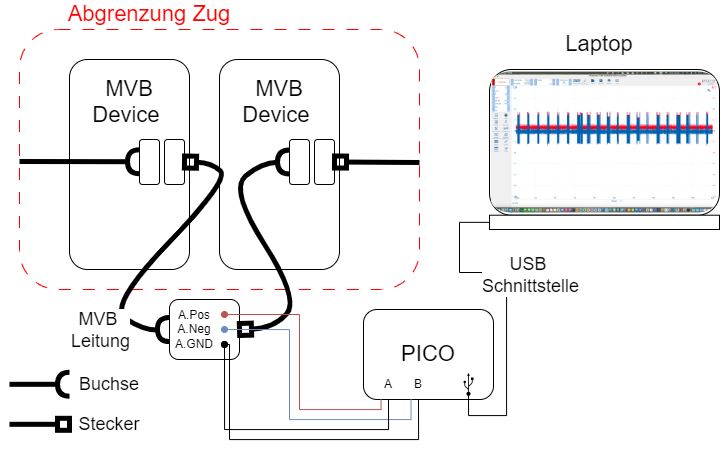
\includegraphics[width=0.8\linewidth]{Figures/Chap3/Busauslastung/Messaufbau_PICO_IC2000.png}
%     \caption{Messaufbau Busauslastung messen}
%     \label{fig:MessaufbauBusauslastungMessen}
% \end{figure}

% Die erfassten Daten wurden anschliessend in das MATLAB-Dateiformat (.mat) exportiert. Die Struktur der MATLAB-Datei ist in Abbildung \ref{fig:MatlabFileStruktur} dargestellt. Die Variablen \textit{A} und \textit{B} entsprechen den Messpunkten des Picoscope, während \textit{Tinterval} die Zeit zwischen zwei Messpunkten angibt. 

% \begin{figure}[H]
%     \centering
%     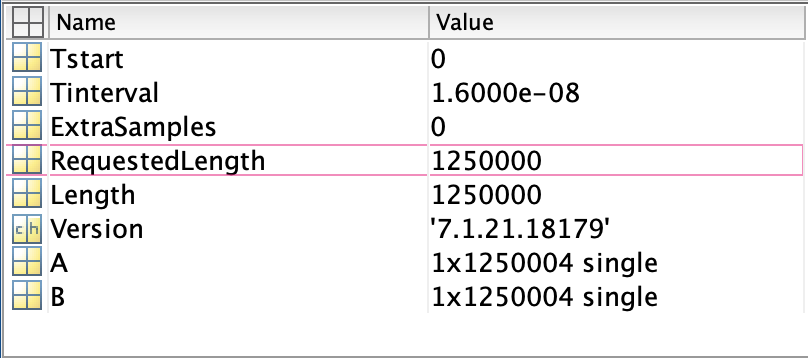
\includegraphics[width=0.5\linewidth]{Figures/Chap3/Busauslastung/Matlab_file_struktur.png}
%     \caption{Matlab File Struktur}
%     \label{fig:MatlabFileStruktur}
% \end{figure}

% Der Messaufbau blieb für die Messungen unter Normallast und Volllast identisch. Um die Volllast zu simulieren, wurde der Befehl zur Anzeige der Depot-Diagnosedaten auf dem Fahrzeugdisplay ausgelöst, bevor die Messung gestartet wurde. Der Zeitraum zwischen der Eingabe des Befehls und der Darstellung der Daten auf dem Display beträgt etwa 5 Sekunden.

% \subsection{Einstellung Osziloskop}
% Das Picoscope-Osziloskop wurde entsprechend der Anforderungen für die Messung wie folgt eingestellt: Die Abtastrate wurde auf 62.5 MS/s eingestellt, wodurch sich ein Abtastintervall von 16ns ergibt. Somit ist sichergestellt, dass jedes Machester-Bit mit jeweils 40 Punkten abgetastet wird (siehe Kapitel \ref{sub:BitEncoding}). Mit dem verfügbaren Speicher des Picoscope lassen sich somit 25 Messungen mit einer Messdauer von 20ms speichern.

% \subsection{Matlab Auswertung}
% Die Auswertung der Analogwerte wurde mit Matlab realisiert. Ziel war es herauszufinden, wie gross die Busauslastung in Bits/s ist. Für die Übertragung mit Bluetooth waren nur die Master Frame Daten und die Master Check Sequenz (siehe Kapitel \ref{sub:MasterFrame}) sowie die Slave Frame Daten und die Slave Check Sequenzen (siehe Kapitel \ref{sub:SlaveFrame}) von Interesse. Der Overhead der Start- sowie der Enddelimiter müssen entfernt werden. 

% \subsubsection{Variablen initialisieren}
% %\textcolor{red}{Zeitvektor initialisiert, damit Signal im Zeitbereich geplotet werden konnte. Analyse des Signals möglich. Einbindung Plot!}
% Die mit Picoscope generierten Matlab Dateien konnte das Signal im Zeitbereich grafisch dargestellt werden. Der unten dargestellte Code zeigt, wie die Abbildung \ref{fig:MvbOhneDds} erstellt wurde. Die Abbildung \ref{fig:MvbMitDds} wurde mit dem anderen Datenset und einem angepassten Titel erstellt. 

% \begin{lstlisting}[language=Matlab]
% load("Messung ohne DDS/20240930-0002_01.mat")
% %load("Messung mit DDS/20240930-0004_18.mat")

% % ---- Variabeln initialisieren --------
% N_org = length(A);          
% Ts = Tinterval;             % gegeben von .mat
% t_org = [0:N_org-1]*Ts;     % erstellung Zeitvektor

% figure()                    % neuer Plot erstellen
% plot(t_org, C)
% title("MVB Signal ohne DDS im Zeitbereich (1 von 25)")
% legend("MVB")
% axis([0 0.02 -7 7])

% % ----- PLOTS ----------------
% plot(t_org, C)              % Plot Signal im Zeitbereich
% \end{lstlisting}

% \begin{figure}[H]
%     \centering
%     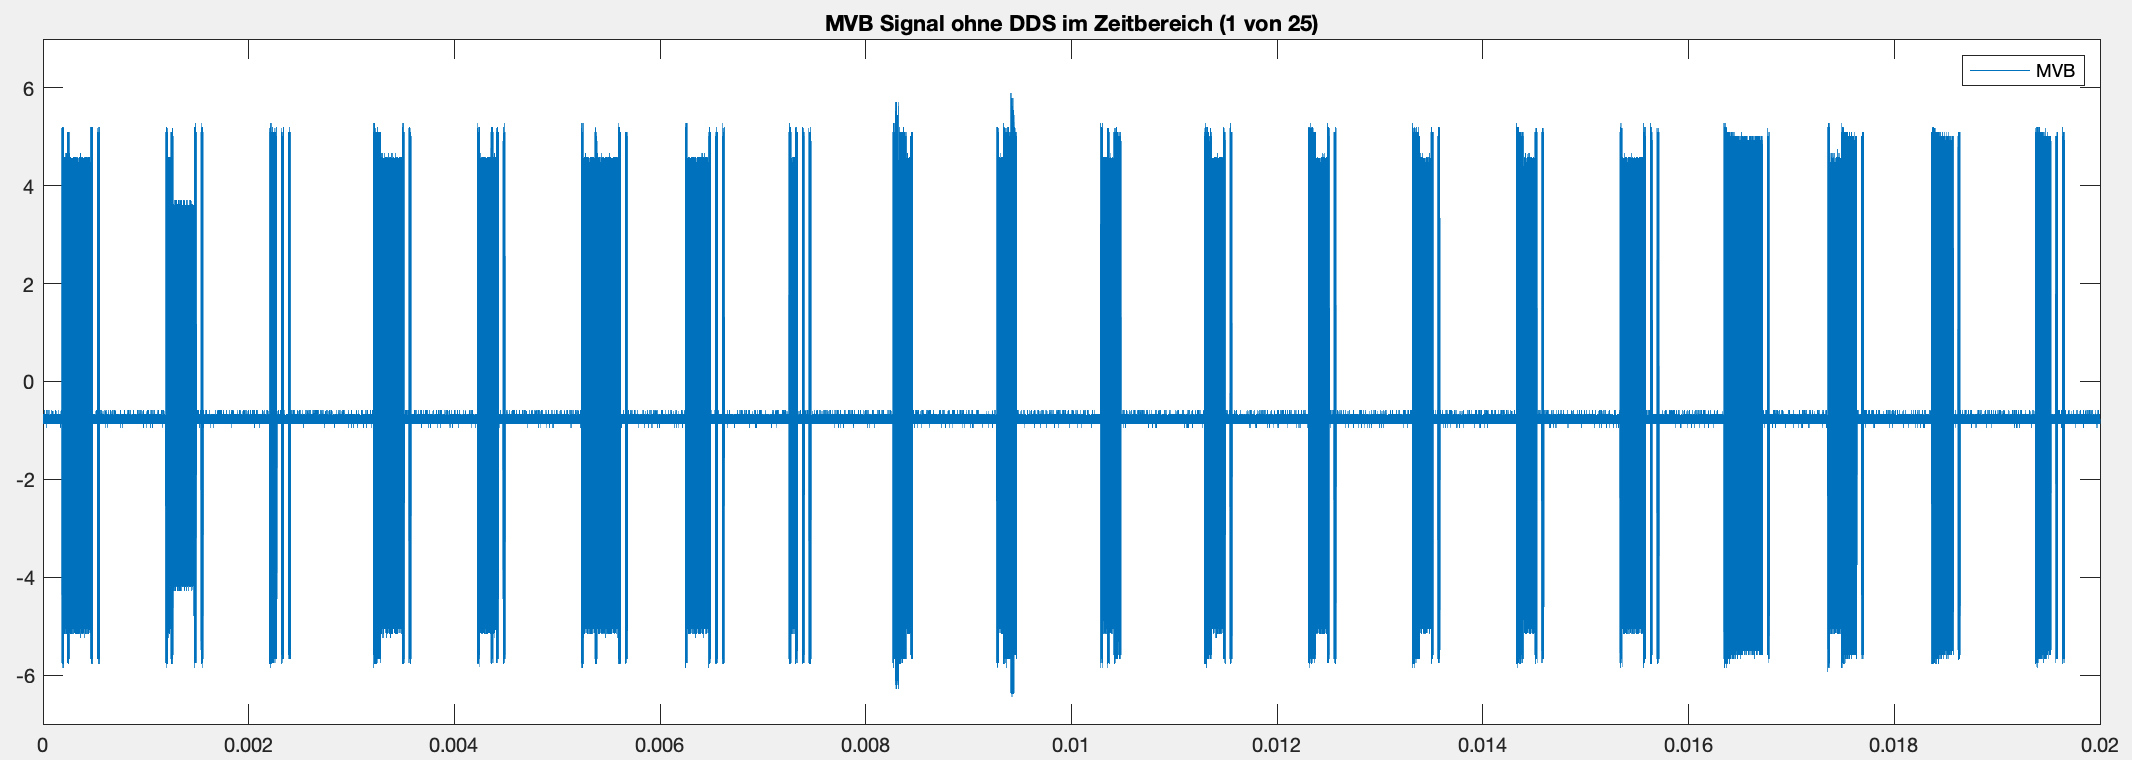
\includegraphics[width=0.8\linewidth]{Figures/Chap3/Busauslastung/MVB_Signal_ohneDDS.png}
%     \caption{MVB Signal ohne DDS, Aufzeichnung 1 von 25}
%     \label{fig:MvbOhneDds}
% \end{figure}

% \begin{figure}[H]
%     \centering
%     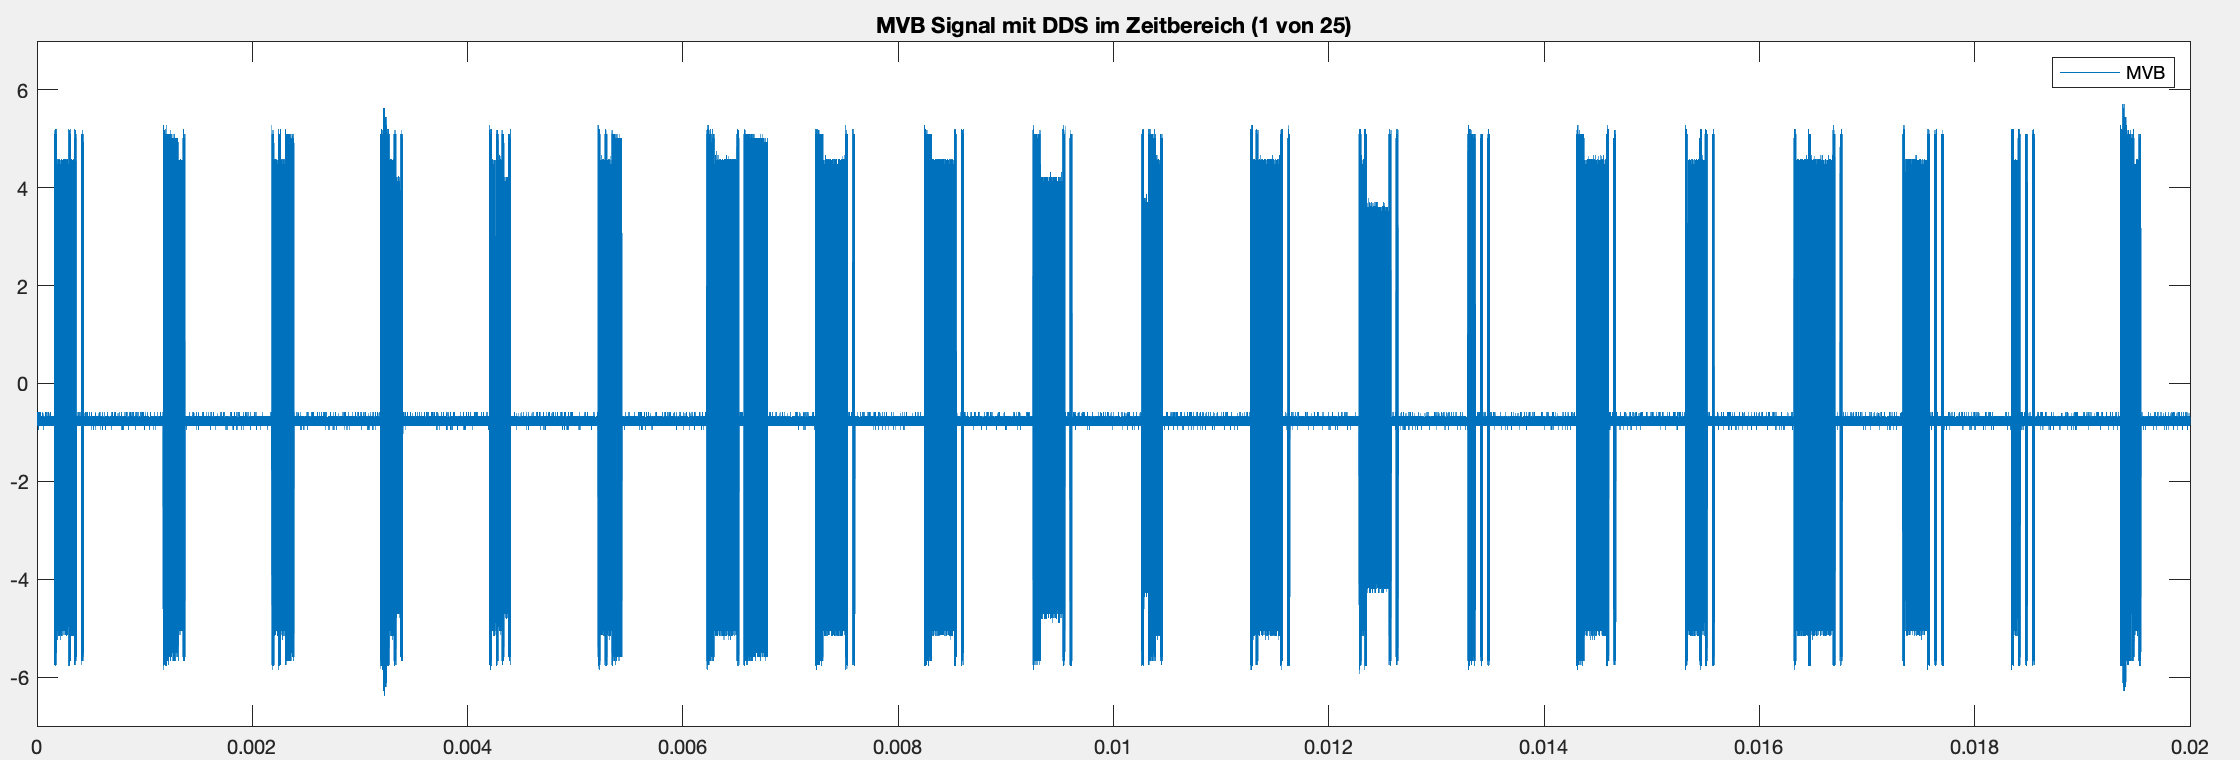
\includegraphics[width=0.8\linewidth]{Figures/Chap3/Busauslastung/MVB_Signal_mitDDS.png}
%     \caption{MVB Signal mit DDS, Aufzeichnung 1 von 25}
%     \label{fig:MvbMitDds}
% \end{figure}

% Zu sehen sind Zeitbereiche, in denen Daten ausgetauscht werden gefolgt von einem Zeitbereich, in dem sich der Bus in einem Idle Zustand befindet. Ebenfalls bemerklich ist, dass von blosem Auge der Unterschied zwischen Volllast (mit DDS) und Normallast (ohne DDS) nicht zu erkennen ist.

% \subsubsection{Delimiter erkennen}
% %\textcolor{red}{Anzahl delimiter erkennen. Charakteristik erkannt -> letzte werte Idle, dann Nulldurchgang, aber nur wenn einer der nächsten 20 Werte über null ist, sonst wurde peak am schluss auch gezählt. }
% Um die Start-Delimiter zu erkennen, wurde die Charakteristik eines Delimiters gemäss Kapitel \ref{sub:StartDelimiter} untersucht. In Abbildung \ref{fig:AusschnittMvbOhneDds} wurde der Zeitbereich vergrössert. Dadurch lassen sich die Telegramme (gemäss Kapitel \ref{sub:MasterSlavePrinzip}) besser sehen.

% \begin{figure}[H]
%     \centering
%     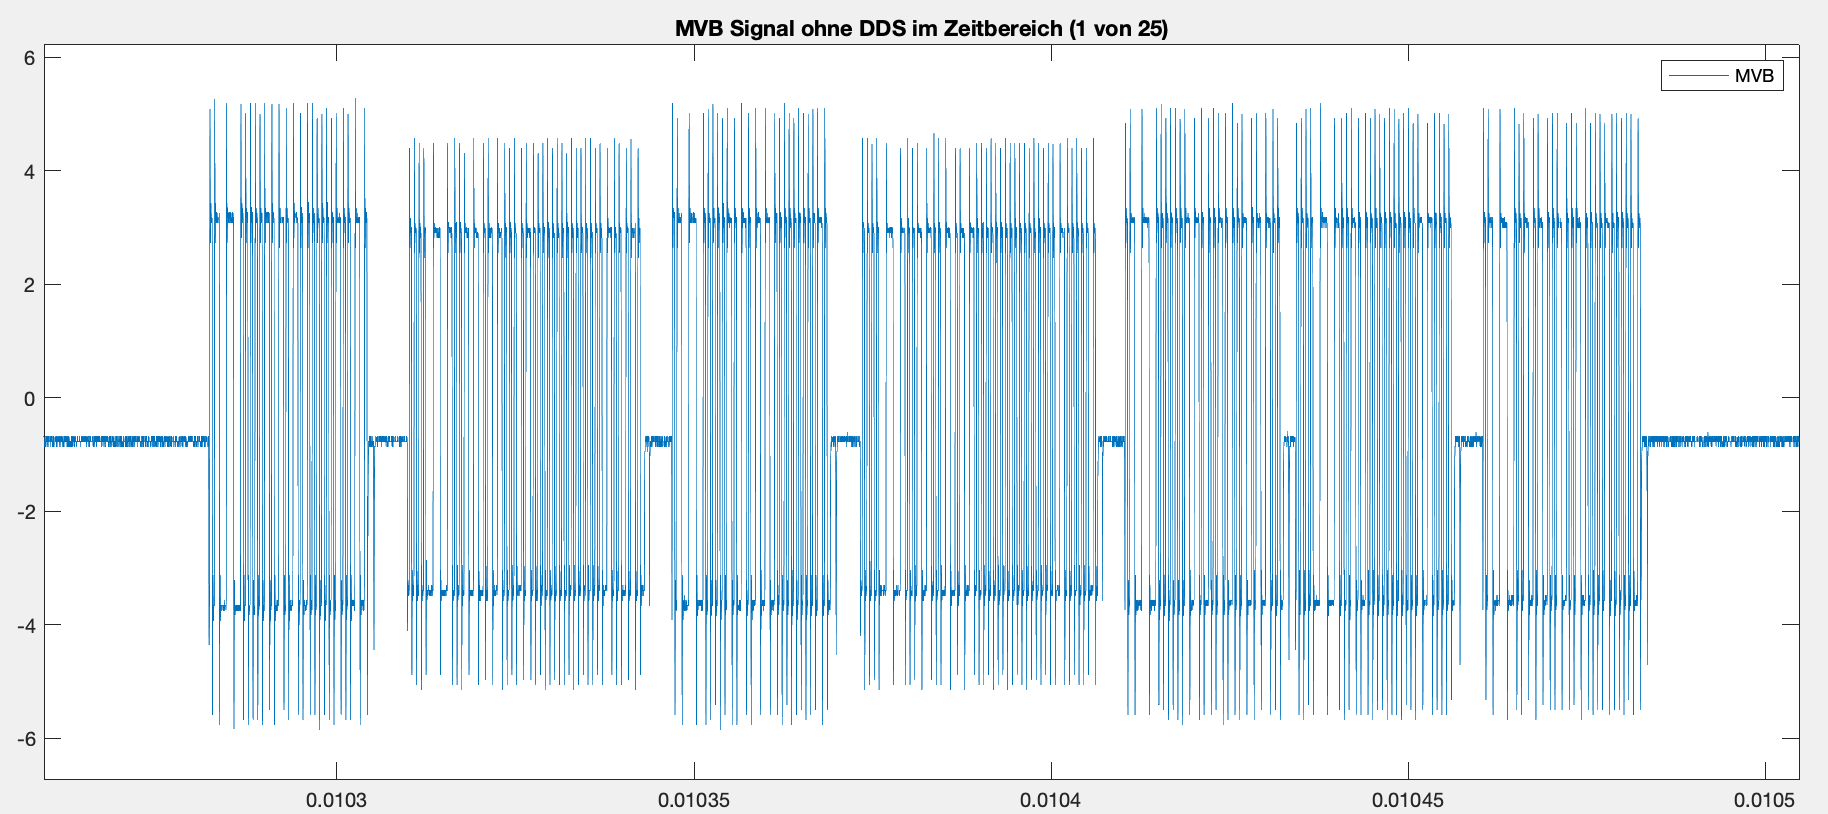
\includegraphics[width=0.9\linewidth]{Figures/Chap3/Busauslastung/Ausschnitt_MVB_ohneDDS.png}
%     \caption{Ausschnitt MVB Signal ohne DDS}
%     \label{fig:AusschnittMvbOhneDds}
% \end{figure}

% Zu sehen ist, dass vor jedem Startbit (Master- und Slave-Frame) das Signal eine gewisse Zeit Idle signalisiert, bevor das Startbit eine negative Flanke auslöst. Das kann verwendet werden, um das Startbit zu erkennen. In einem Array mit 20 Werten sollen alle Werte im Idle Bereich liegen (zwischen -0.5 und -1 V) und die nächste negative Flanke, also ein Wert unter -1 wird als Start detektiert. Für die Ausgabe auf dem Plot wurden die Spannungs- und Zeitpunkte gespeichert und dem Plot hizugefügt. Abbildung \ref{fig:MVBDelimiterFalsch} zeigt diesen Plot.

% \begin{lstlisting}[language=Matlab]
% detected_values = [];
% detected_times = [];
% delimiter = 0;

% n_samples = 20;

% for i = n_samples+1:length(C)
%     % Ueberpruefen, ob die letzten 20 Werte zwischen -0.5 und -1 liegen
%     if all(C(i-n_samples:i-1) > -1 & C(i-n_samples:i-1) < -0.5)

%         % Wenn der naechste Wert kleiner als -1.0 ist
%         if C(i) < -1.0
%             % Zaehler erhoehen
%             delimiter = delimiter + 1;
                
%             % Speichern des Werts und des entsprechenden Zeitwerts
%             detected_values = [detected_values, C(i)];
%             detected_times = [detected_times, t_org(i)];
%         end
%     end
% end
% \end{lstlisting}

% \begin{figure}[H]
%     \centering
%     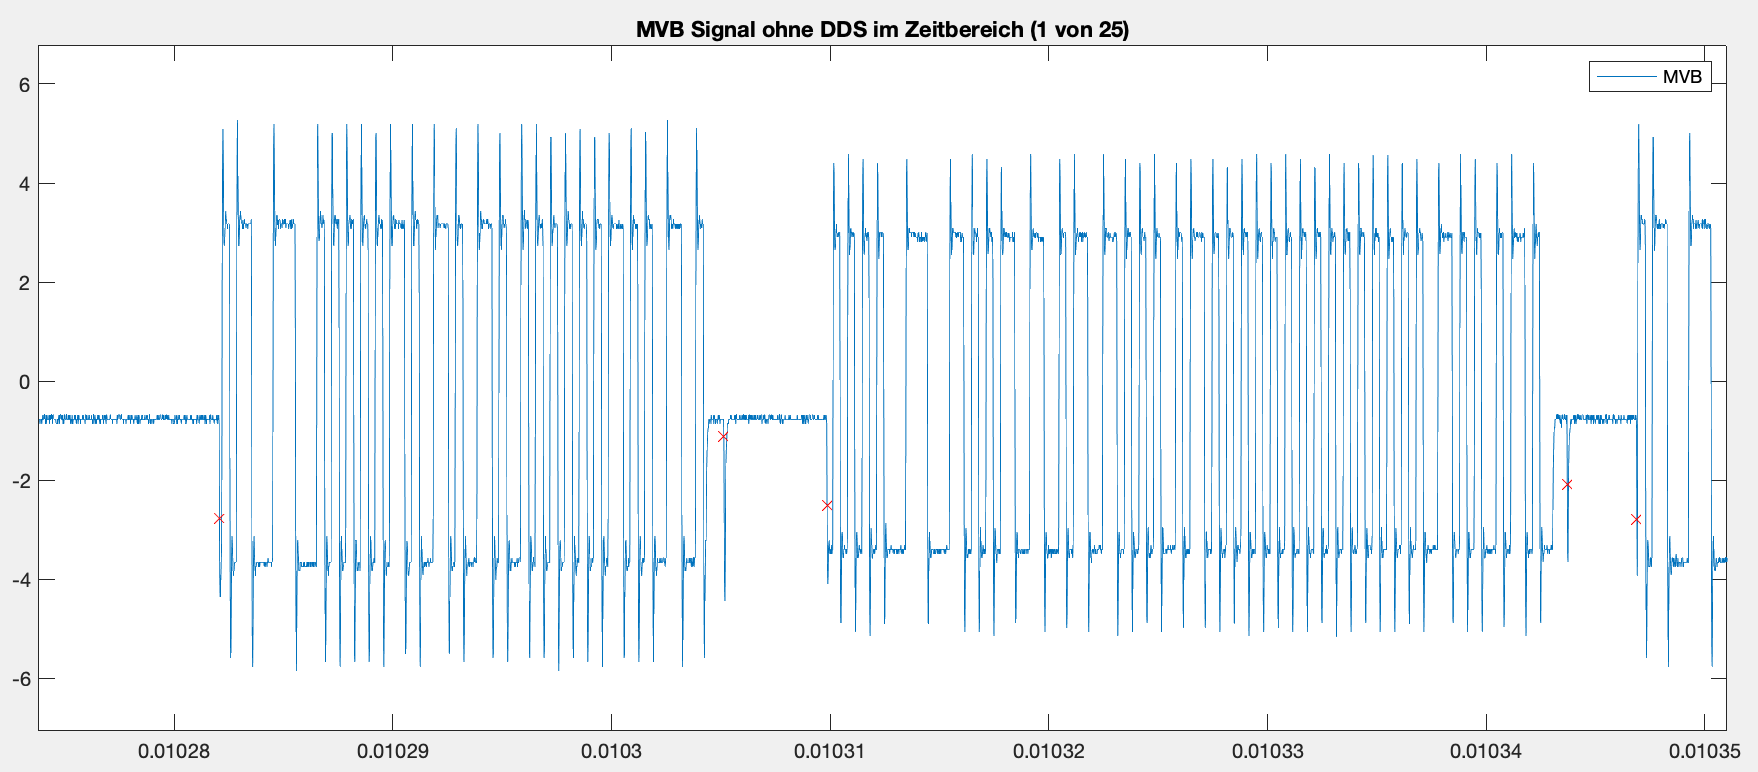
\includegraphics[width=0.9\linewidth]{Figures/Chap3/Busauslastung/Ausschnitt_MVB_Delimiter_falsch.png}
%     \caption{Ausschnitt der MVB Messung ohne DDS mit nicht korrekter Delimiter erkennung}
%     \label{fig:MVBDelimiterFalsch}
% \end{figure}

% Wird der Zeitbereich erneut vergrössert, ist zu sehen, dass am Ende eines Master- oder Slave-Frame die Signalleitung in den negativen Bereich gezogen wird, was zu einer falschen erneuten Detektion eines Start-Delimiters führt.

% Das Startbit hat gemäss Kapitel \ref{sub:StartDelimiter} die Eigenschaft, dass es während der ersten Hälfe der Bitdauer High und in der zweiten Hälfte Low ist. Dies kann als Bedingung für die Erkennung der eines Start-Delimiters einfliessen. Dies wurde im Code so implementiert, dass nach der Erkennung der negativen Flanke zusätzlich abgefragt wurde, ob einer der nächsten 20 Werte (also 333ns) ein Wert über 0V gemessen wurde. Der wurde Code wie folgt angepasst und der daraus entstandene Plot ist in Abbildung \ref{fig:DelimiterRichtig} zu sehen.

% \begin{lstlisting}[language=Matlab]
% detected_values = [];
% detected_times = [];
% delimiter = 0;

% n_samples = 20;

% for i = n_samples+1:length(C)
%     % Ueberpruefen, ob die letzten 20 Werte zwischen -0.5 und -1 liegen
%     if all(C(i-n_samples:i-1) > -1 & C(i-n_samples:i-1) < -0.5)

%         % Wenn der naechste Wert kleiner als -1.0 ist
%         if C(i) < -1.0

%             % Wenn einer der naechsten 20 Werte ueber Null ist, ist es ein Start Delimiter
%             if any(C(i+1:i+20) > 0)
            
%                 % Zaehler erhoehen
%                 delimiter = delimiter + 1;
                    
%                 % Speichern des Werts und des entsprechenden Zeitwerts
%                 detected_values = [detected_values, C(i)];
%                 detected_times = [detected_times, t_org(i)];
                
%             end
%         end
%     end
% end
% \end{lstlisting}

% \begin{figure}[H]
%     \centering
%     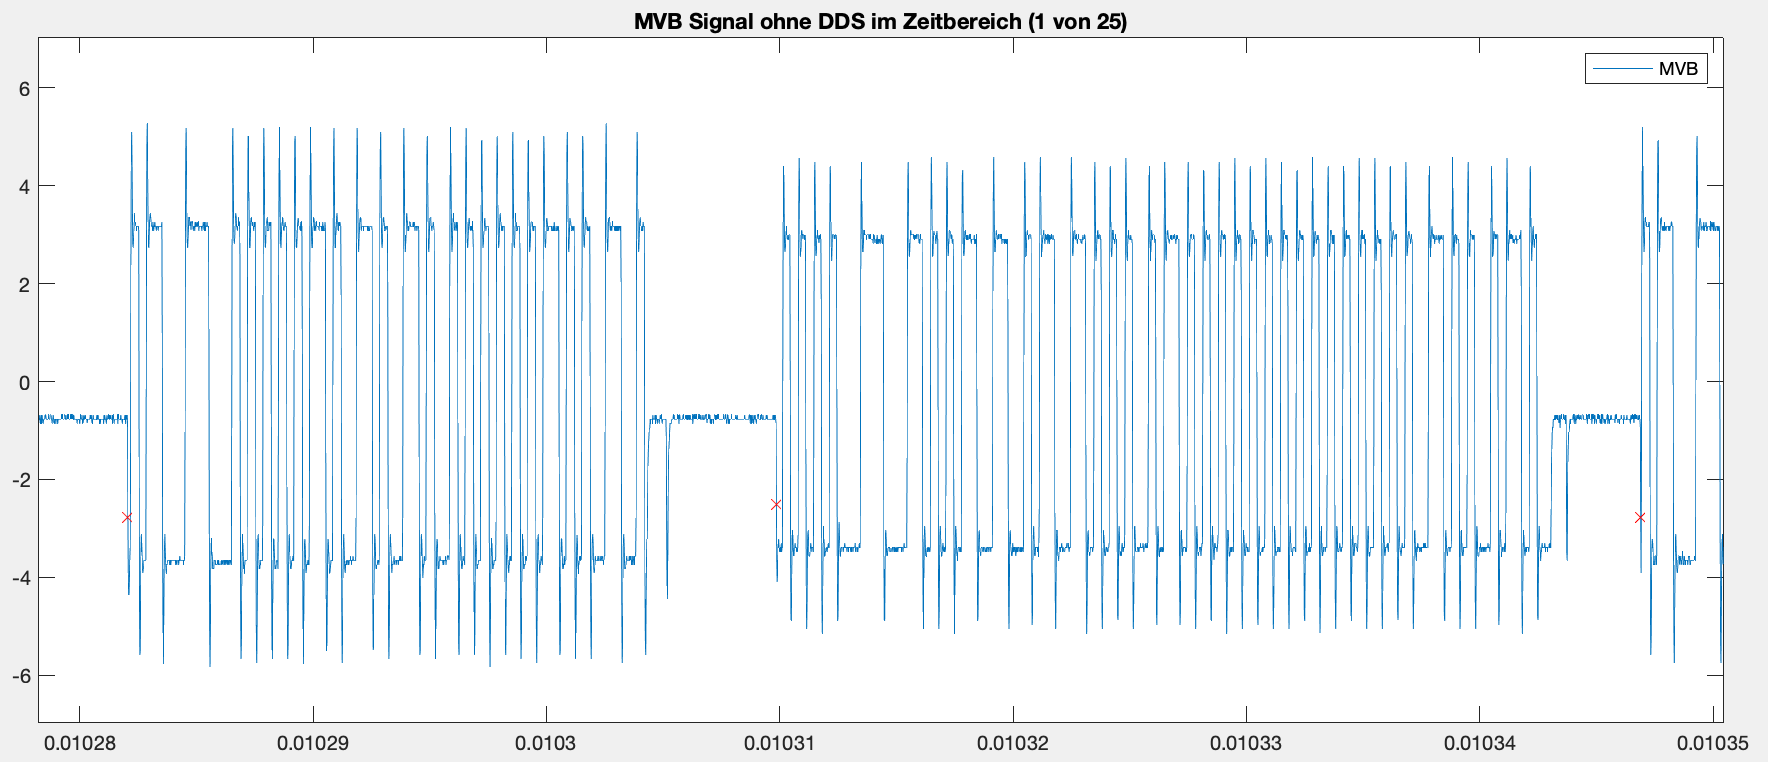
\includegraphics[width=0.9\linewidth]{Figures/Chap3/Busauslastung/Ausschnitt_MVB_Delimiter_richtig.png}
%     \caption{Ausschnitt der MVB Messung ohne DDS, mit korrekter Start-Delimiter erkennung}
%     \label{fig:DelimiterRichtig}
% \end{figure}


% \subsubsection{Nulldurchgänge}
% \label{subsub:Nulldurchgänge}
% %\textcolor{red}{Anzahl bits mit Startdelimiter erkennen. Als erstes alle werte zwischen 0 und -1V gelöscht, weil Idle. Dann wurde eine Flanke detektiert. Wenn eine Flanke detektier um 30 Werte vorwärts springen (damit zweite Flange nicht nochmals erkennt wird (manchester encodiertes Signal)}
% In diesem Schritt wurde mit Matlab versucht, die Anzahl Bits zu aus der Messung auszuwerten. Gemäss Kapitel \ref{sub:BitEncoding} gibt es für den Wert "'0"' und "'1"' jeweils einen Flankenwechsel in der Hälfte der Bitdauern (abk. BT und entspricht gemäss Kapitel \ref{sub:GeschwindigkeitDatenbus}: 1 BT = 666ns). Dies kann verwendet werden, um die Anzahl Bits herauszufinden. Anhand Abbildung \ref{fig:Suchalgo_Bits} kann der gewählte Suchalgorithmus erklärt werden.

% \begin{figure}[H]
%     \centering
%     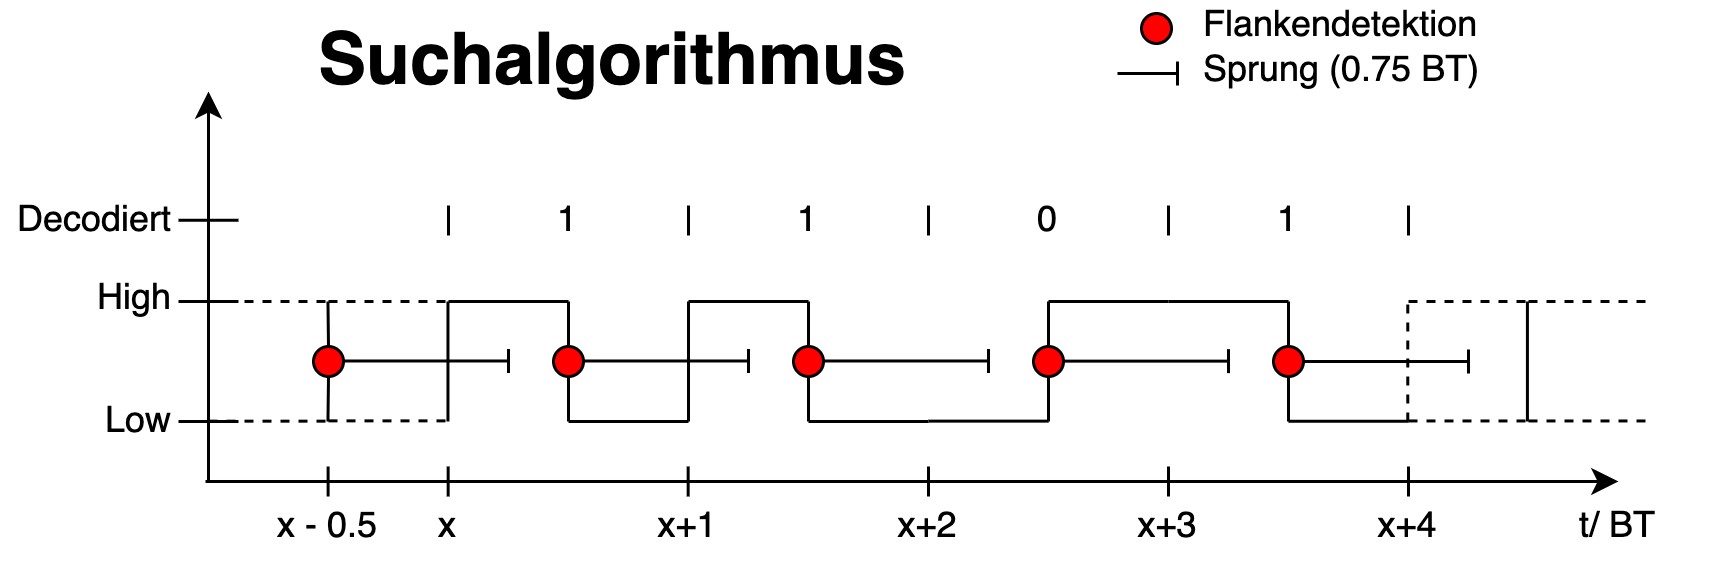
\includegraphics[width=0.9\linewidth]{Figures/Chap3/Busauslastung/Suchalgorithmus_Bits.png}
%     \caption{Suchalgorithmus der Bits in einem Manchester encodierten Signal}
%     \label{fig:Suchalgo_Bits}
% \end{figure}

% X steht dabei für einen zufälligen Zeitpunkt. Auf der Abszisse ist die Zeit in Bitdauer aufgetragen. Auf der Ordinate ist einmal ein Beispielsignal und die Decodierung vom Signal aufgezeigt. Da in der Mitte der Bitdauer eine Flanke zu erwarten ist, wird auch eine halbe Bitdauer vor X eine Flanke erwartet. Dies ist der Einstieg. Wird eine Flanke detektiert, wird um eine Bitdauer von 0.75 positiv in der Zeit gesprungen. Der Sprungpfeil zeigt mit seinem flachen Ende, ab wo die nächste Flanke gesucht wird. Der Sprung hat den Grund, dass Flankendetektionen, wie dieser bei \textit{x+1} in Abbildung \ref{fig:Suchalgo_Bits}, nicht gezählt werden, da diese die Auswertung verfälschen.

% Gemäss Abbildungen \ref{fig:MasterStartdel} und \ref{fig:SlaveStartdel} sind die Anzahl Flanken, welche in einem Master Startdelimiter und einem Slave Startdelimiter gezählt werden gleich Sieben.

% \begin{figure}[H]
%     \centering
%     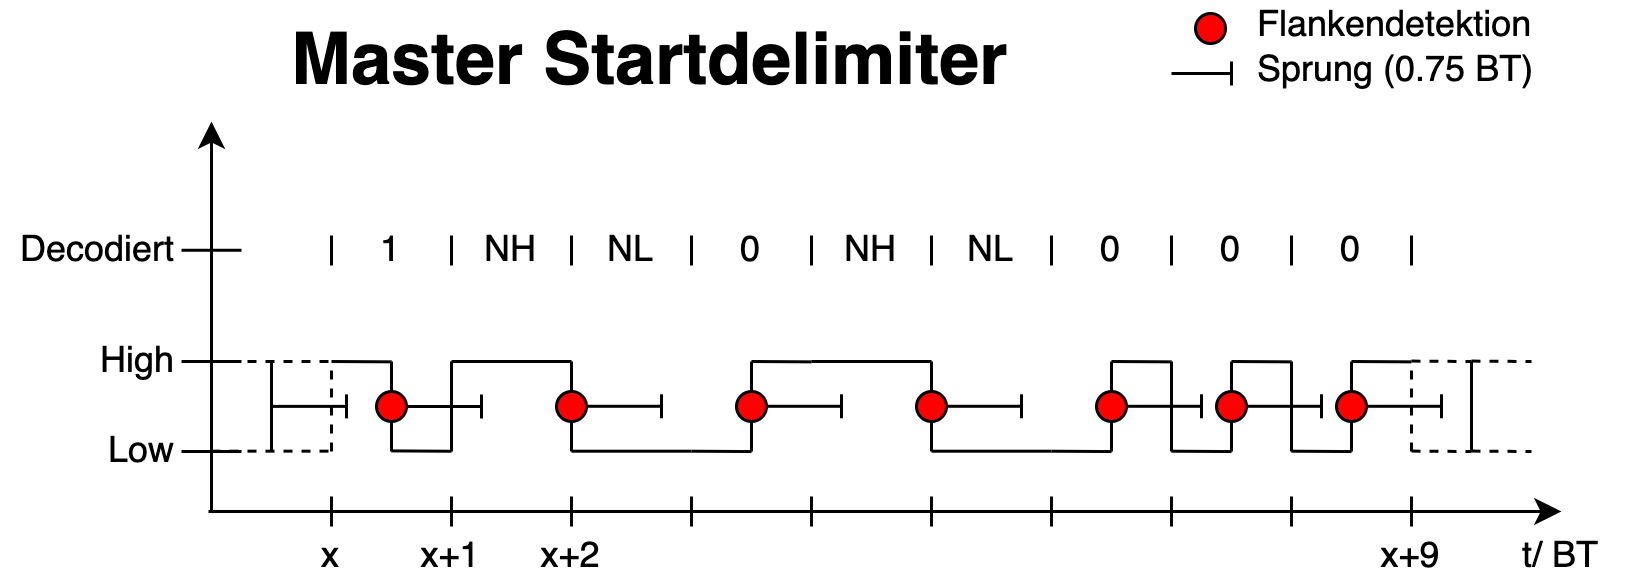
\includegraphics[width=0.9\linewidth]{Figures/Chap3/Busauslastung/Master_Startdel.png}
%     \caption{Anzahl Flanken in einem Master Startdelimiter}
%     \label{fig:MasterStartdel}
% \end{figure}

% \begin{figure}[H]
%     \centering
%     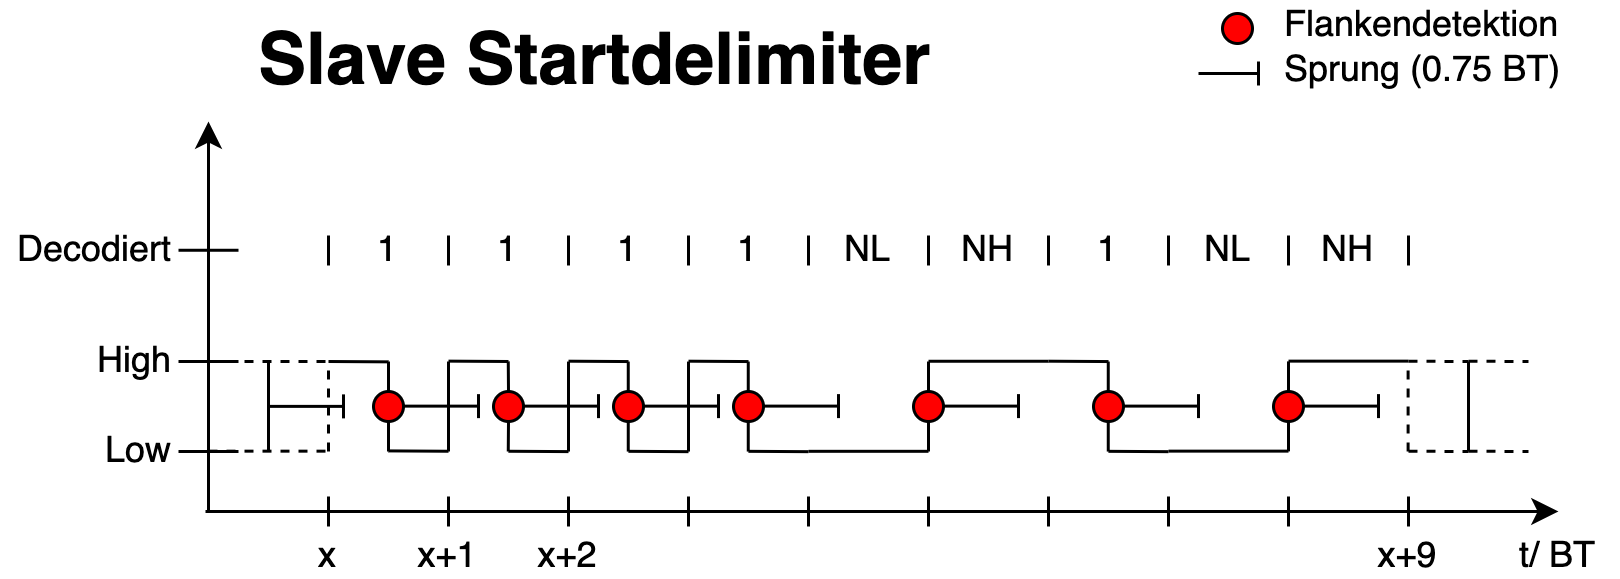
\includegraphics[width=0.9\linewidth]{Figures/Chap3/Busauslastung/Slave_Startdel.png}
%     \caption{Anzahl Flanken in einem Slave Startdelimiter}
%     \label{fig:SlaveStartdel}
% \end{figure}


% Für die Auswertung am MVB Signal wurde in einem ersten Schritt das Idle Signal, also alle Messpunkte zwischen -0.5 V und -1V aus dem Signal entfernt. Was daraus folgt, ist ein Signal, welches Startbits, Startdelimiter, Masterframe- sowie Slaveframe-Daten enthält. In Abbildung \ref{fig:ReineDaten} ein Vergleich zwischen beiden Signalen zu sehen. Oben mit Idle Signal, unten ohne Idle Signal.

% \begin{figure}[H]
%     \centering
%     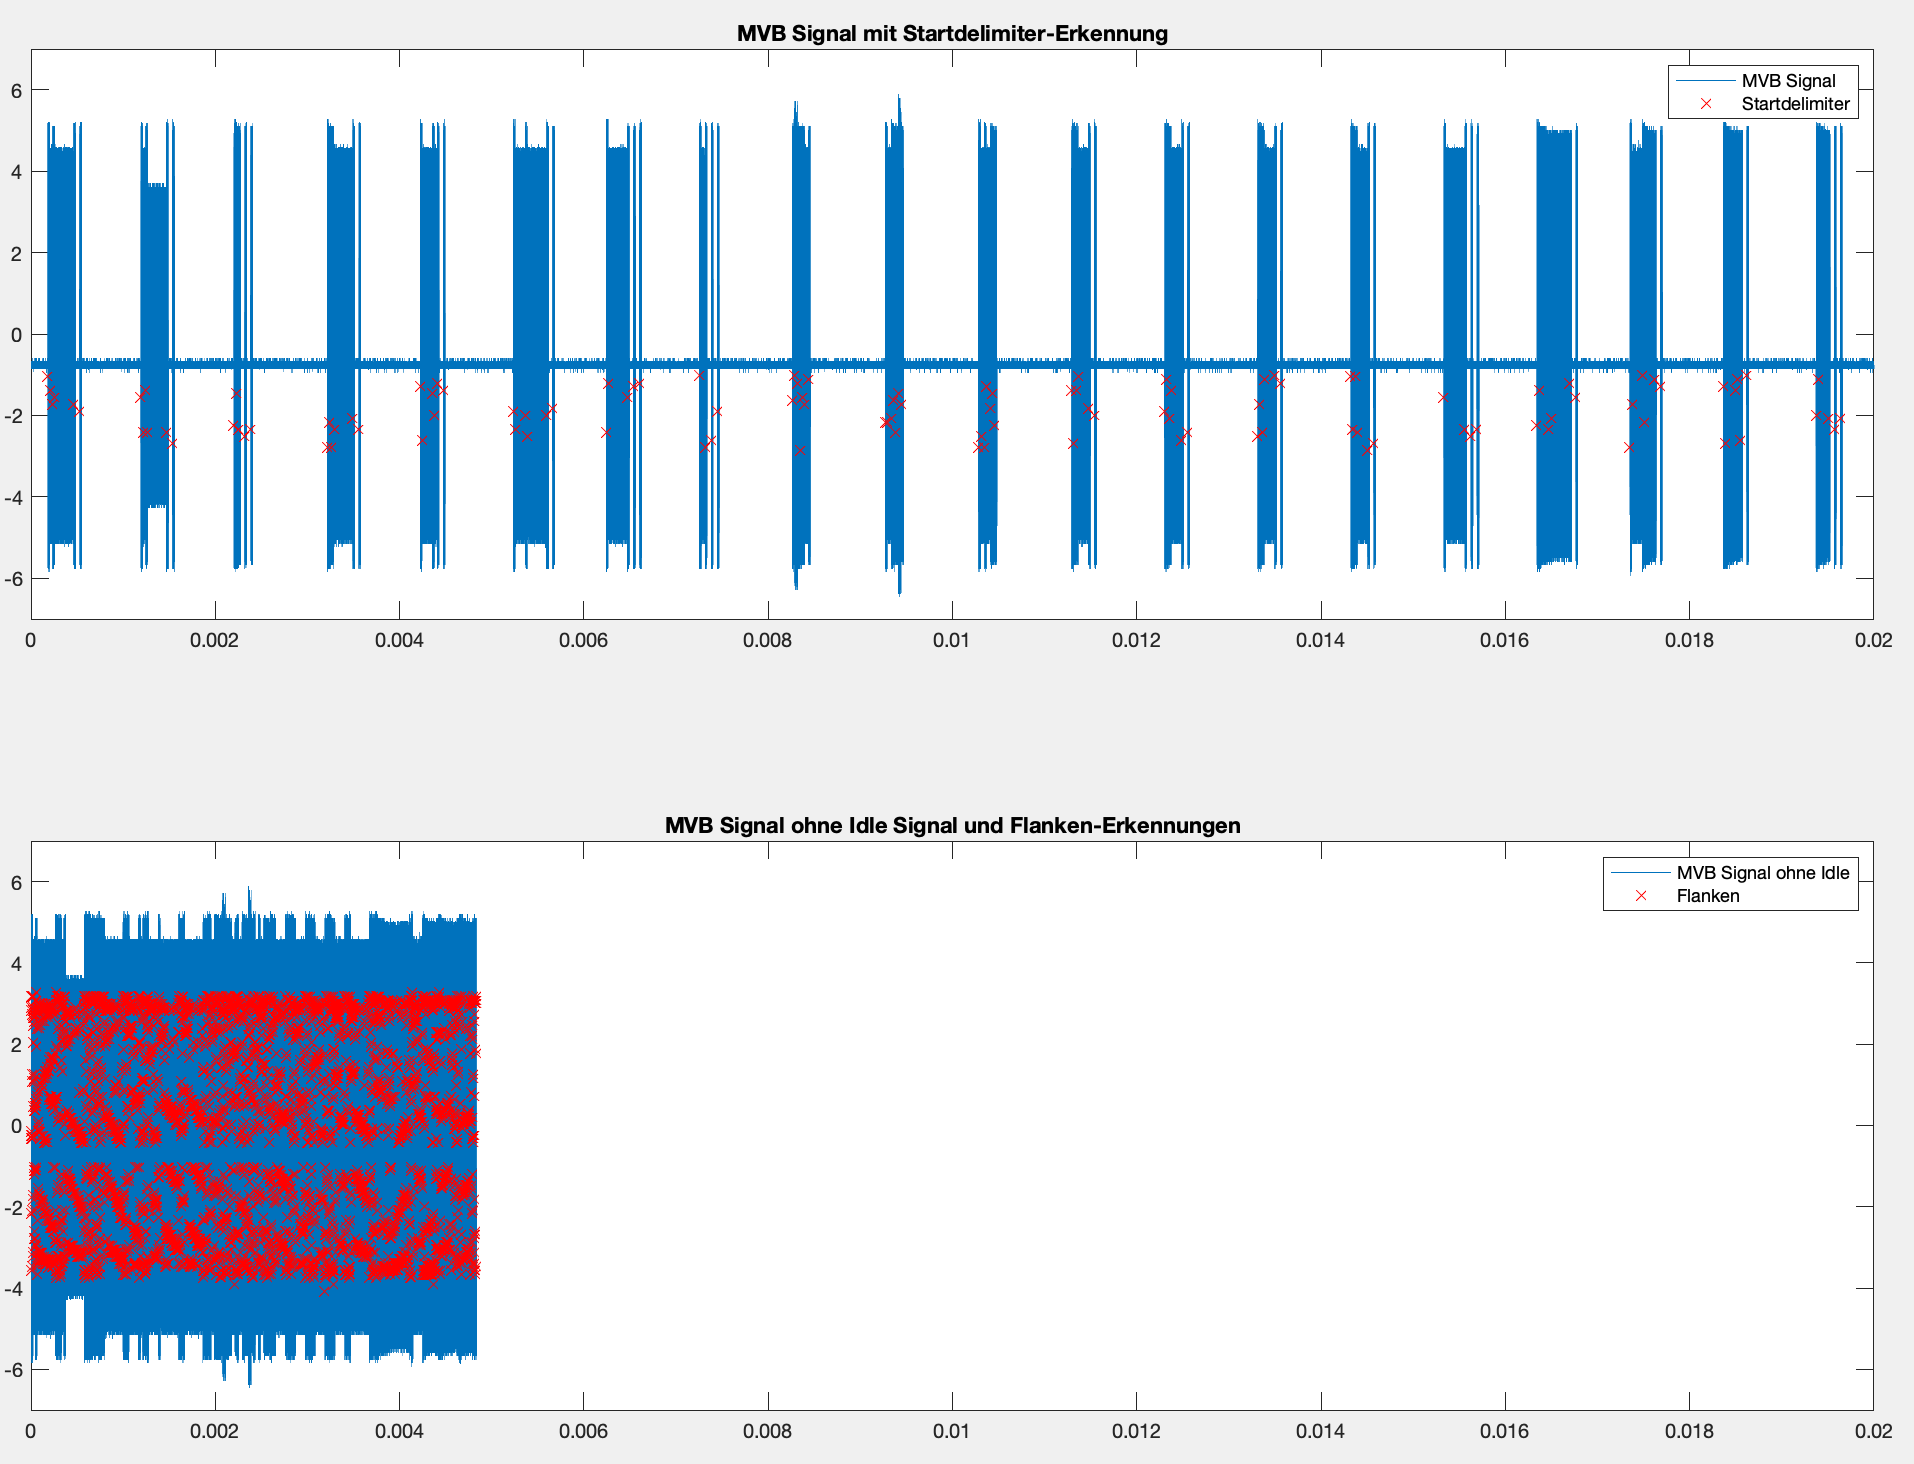
\includegraphics[width=0.75\linewidth]{Figures/Chap3/Busauslastung/Vergleich_MVB_mit_ohne_Idle.png}
%     \caption{Vergleich MVB Signal mit und ohne Idle Signal über einen Zeitraum von 20ms}
%     \label{fig:ReineDaten}
% \end{figure}

% Der Suchalgorithmus wurde in Matlab gemäss dem nachfolgenden Code implementiert

% \begin{lstlisting}[language=Matlab]
% % ---- Nulldurchgaenge ---------------

% % Aus dem Sigal, nehme alle Werte ausser das Idle Signal (~ -0.75V)
% data_ohne_idle = C(C > -0.5 | C < -1);

% % neuer Zeitvektor initalisieren
% N_fil = length(data_ohne_idle);
% t_fil = [0:N_fil-1]*Ts;

% % Zaehlervariablen initialisieren
% z_num = 0; % Zaehlervariable fuer bit == flanken
% used_i = [];

% % Starte bei Index 10, damit wird erste Fanke des Startbits uebersprungen
% i = 10; 


% while i < N_fil

%     % Positive Flanke erkennen
%     if data_ohne_idle(i) < 0.75 && data_ohne_idle(i+1) > 0.75

%         % Fuer Ausgabe in Plot speichern
%         used_i = [used_i , i];
%         z_num = z_num + 1; 

%         % Ueberspringe Manchester Flankenwechsel ( 333ns < t < 666ns; ts = 16ns --> i = i + 20...40)
%         i = i + 30; 

%     % Negative Flanke erkennen
%     elseif data_ohne_idle(i) > 0.75 && data_ohne_idle(i+1) < 0.75

%         % Fuer Ausgabe in Plot speichern
%         used_i = [used_i , i]; 
%         z_num = z_num + 1;

%         % Ueberspringe Manchester Flankenwechsel ( 333ns < t < 666ns; ts = 16ns --> i = i + 20...40)
%         i = i + 30; 
       
%     % Wenn keine Flanke erkennt wird um 1 erhoehen
%     else
%         i = i + 1;
%     end
% end
% \end{lstlisting}




% \subsubsection{Auswertung Effektive Nutzdaten}
% %\textcolor{red}{Effektive = Anzahl Nuldurchgänge - (Delimiert * 9); Tablle effiktive Nutzwerte mit und ohne DDS.}
% Nun wurde ausgewertet, wie viele Bits in einer Zeitdauer von 20ms geschickt wurde und wie viele Startdelimiter in derselben Zeit erkennt wurden. Gemäss Kapitel \ref{subsub:Nulldurchgänge} ist sind die Master-Startdelimiter und Slave-Startdelimiter sieben Bits gross. Dies kann mit der Anzahl delimiter multiliziert werden und von der gesammtsumme der gezählen Bits abgezogen werden. Im nachfolgenden Code wird gezeigt, wie das in Matlab realisiert wurde.

% \begin{lstlisting}[language=Matlab]
% % --- Auswertung

% dlm = delimiter * 7; % Delimiter bits (master/slave)
% eff_bps = (z_num - dlm)/0.02; % Bits pro Sekunde effektive Nutzdaten

% \end{lstlisting}

% Die Busauslastung wurde für jede der je 25 Messungen für Normallast und Volllast durchgeführt. Der Matlabcode dazu ist im Anhang \ref{XX} zu finden. In Tabelle \ref{tab:Busauslastung} ist die Auswertung  der Busauslastung tabellarisch dargestellt. Die Spalten \textit{min} und \textit{max} sind jeweils die minimal sowie maximalen Werte der je 25 Messungen. Die Spalte \textit{mean} wurde mit dem Matlabbefehl \textit{mean()} berechnet und gibt den Mittelwert über die je 25 Messungen aus. 

% \begin{table}[H]
%     \centering
%     \begin{tabular}{r|c|c|c}
%         & min in Bits/s & mean in Bits/s & max in Bits/s\\ 
%         \hline
%         Normallast & 2.4705e+05 & 2.8823e+05 & 3.1885e+05\\
%         \hline
%         Volllast & 2.5935e+05 & 3.0456e+05 & 4.204e+05 \\
%     \end{tabular}
%     \caption{Busauslastung mit und ohne DDS. }
%     \label{tab:Busauslastung}
% \end{table}


% %----------------------------------------------------------------------
% % SECTION Wahl der Hardware
% %----------------------------------------------------------------------

% \section{Design eigener Sniffer}
% Für den ersten Entwurf des Sniffers wurde eine Anforderungsliste erstellt, in welcher die Fest- wie auch Wunschanforderungen definiert wurden. In einem ersten Entwurf wurde schematisch dargestellt in welcher Reifenfolge, welche Aufgabe von welcher Hardware durchgeführt werden soll. 

% Dieser schematische Entwurf (siehe Abbildung \ref{fig:AufbauSniffer}) zeigt die verwendete Hardware auf und wie diese untereinander verbunden sind. Dabei wurden direkt die technischen Anforderungen, welche durch den MVB vorgegeben sind, im Schema dargestellt.

% \begin{figure}[H]
%     \centering
%     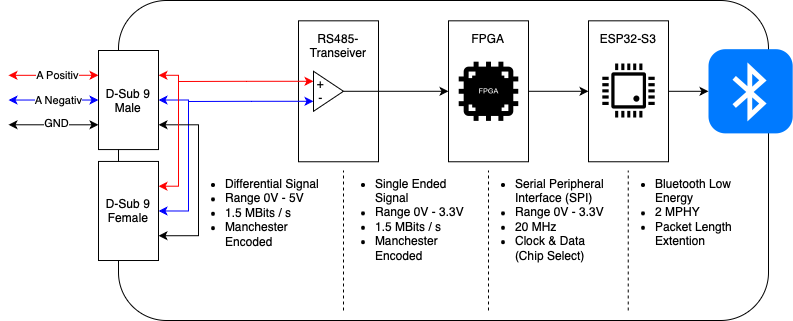
\includegraphics[width=0.8\linewidth]{Figures/Chap3/Design Eigener Sniffer/Aufbau_Sniffer.png}
%     \caption{Schematischer Aufbau Sniffer}
%     \label{fig:AufbauSniffer}
% \end{figure}

% Um aus dem Differenziellen Manchestersignal vom MVB ein Digitales Signal, welches 0v bei einer Negativen Flanke und 3.3V bei einer Positiven Flanke annehmen soll, zu erzeugen wurde ein RS485 Transceiver verwendet. Der Transceiver wird mit einer Spannung von 3.3V versorgt. Das erzeugte digitale Signal vom RS485 wird weiter ins FPGA (Field Programmable Gate Array) geleitet, wo der Manchestercode decodiert wird und als Bitstream über das SPI an den Mikrocontroller ESP32 gesendet wird. der Mikrocontroller wertet die Daten aus und gibt diese dann per Bluetooth aus.

% In einer Prototypenphase und somit auch im Rahmen der Projektarbeit, sind dafür drei verschiedene Evaluationsboards verwendet worden. Das definierte Ziel für den fertigen Sniffer ist es ein eigenes PCB zu erstellen, welche die benötigten Bauteile auf einem Board vereint. Ebenfalls soll der fertige Sniffer ein schützendes und abschliessendes Gehäuse, mit den nötigen Ausschnitten besitzen.

% \subsection{Wahl der Hardware}
% In den folgenden Kapitel wird erläutert warum diese Hardware für den MVB-Sniffer gewählt wurde. Im Kapitel \ref{} wird die Wahl der Hardware nochmals abschliessend diskutiert und allfällige Änderungen in der Wahl als Ausblick festgehalten.

% \subsubsection{RS485}
% Der RS485 Transceiver macht aus einem differentiellen Signal ein Digitales Signal, welches zwischen der Speisespannung und 0V hin und her wechselt. Das Ausgangssignal kann dann im Falle des MVB von Busteilnehmern ausgewertet werden. Da im Anwendungsbereich des MVB (ESD) auf den Schienenfahrzeugen, für welche der Sniffer ausgelegt wird, bereits RS485 Transceiver eingesetzt werden, war es naheliegend und sinnvoll diese auch für den Sniffer einzusetzen.

% \subsubsection{FPGA}
% In einer ersten Recherche war eine Lösungsvariante, die Decodierung des Manchestersignal in einer reinen Hardwarelösung wie sie in Abbildung \ref{} zu sehen ist umzusetzen. Als eine weitere Variante wurde dann das FPGA zur Umsetzung des Decoders in Anbetracht gezogen.
% Der Entscheid für den FPGA und gegen die, nicht programmierbare, reine Hardwarelogik, lag in folgenden Punkten:
% \begin{itemize}
%   \item Die Logik des FPGA ist flexibel und schnell anpassbar.
%   \item Das FPGA kann weiter konfiguriert werden um bei einer Weiterentwicklung des Sniffers, weitere Aufgaben Problemlos zu implementieren.
%   \item Das Interesse einen FPGA und dessen Programmierung in VHDL näher kennen zu lernen war gross und in diesem Projekt sicherlich gut realisierbar.
% \end{itemize}


% \subsubsection{SPI}
% Für die Kommunikation zwischen FPGA und ESP32 wurde das Protokoll SPI gewählt, weil es diese Kommunikation möglich macht gleichzeitig zu schreiben und aber auch Daten zu empfangen, SPI ist \textit{"'Full Duplex"'}. Des weiteren können mit diesem Übertragungsprotokoll sehr hohe Raten erreicht werden, welche bei der berechneten Busauslastung (siehe Kapitel \ref{fig:MessaufbauBusauslastungMessen}) von Vorteil ist. Alternativ hätten weitere Protokolle gewählt werden können. zum Beispiel 

% \textcolor{red}{Tabellarischer Vergleich mit anderen Protokollen und Erläuterung wird noch eingefügt}


% \subsubsection{ESP32}
% \textcolor{red}{Warum wurde der µKontroller ESP32 gewählt?}



% %----------------------------------------------------------------------
% % SECTION Hardware FPGA

% %Themen nach Signalfluss aufbauen
% %----------------------------------------------------------------------

% \section{Hardware FPGA}
% Das Field Programmable Gate Array soll die Umwandlung des Manchestersignal vom MVB, bzw. des Signals nach dem RS485 Transceiver, in einen Bitstream realisieren. 

% Die Konfiguration für das FPGA wurde in der Hardwarebeschreibungssprache VHDL geschrieben. Dabei wurden mehrere Dateien für die verschiedenen Aufgaben des FPGA erstellt, um eine saubere und simple Dateistruktur zur erreichen.

% Der Code ist in fünf Dateien aufgeteilt. Zwar wurde dieser in seine verschiedenen Aufgaben, der Decodierung des Signals (Kapitel \ref{Manchester Decodierung}), der Ausgabe des Bitstream auf SPI (Kapitel \ref{SPI}), der Erzeugung der Taktfrequenz für die Abtastung des Manchestersignal, dem Puffern der Werte nach der Abtastung und zuletzt wurde eine Top-Level Datei erstellt um all diese Prozesse zu verknüpfen und die Ein- und Ausgänge des FPGA zu konfigurieren.

% In den folgenden Unterkapiteln werden die einzelnen wichtigsten Prozesse genauer erklärt. 

% \subsection{Manchester Decodierung}
% \label{Manchester Decodierung}
% Zur Decodierung des Manchestersignal, soll jede Flanke vier mal abgetastet werden. Um dies zu realisieren wurde mit der Designsoftware Quartus, in welcher die VHDL-Dateien geschrieben und synthetisiert werden, eine Taktfrequenz von 12 MHz generiert. Was somit acht mal schneller ist als das Manchestersignal des MVB. Folglich werden pro Flanke jeweils vier Werte abgetastet.
% %Die abgetasteten Werte werden fortlaufend in ein acht Bit grosses Register \textit{reg\_sample} geschrieben.
% In Abbildung \ref{} \textcolor{red}{Bild des Signals mit Abtastungspunkte einfügen} ist zum Beispiel das Master Start-Frame mit den jeweiligen Abtastungspunkten in farbe?? zu sehen. %Immer nach acht Zyklen werden die Daten in diesem Register ausgewertet.

% \subsubsection{Auswertung Manchestersignal}
% \label{Auswertung Manchestersignal}
% Immer zu Beginn eines Frame (Master wie auch Slave) wird der Start mit einem Start bit signalisiert, wie bereits in Kapitel \ref{sub:StartDelimiter} beschrieben.
% Sobald das \textit{Start bit} im Auswerteprozess erkannt wird, heisst sobald Bit 5 - 2 im Register \textit{reg\_sample} den Wert \textit{"'1100"'} haben, wechselt das FPGA vom Zustand \textit{IDLE} in den Zustand \textit{RECEIVING}. In diesem Zustand werden Fortlaufend die abgetasteten Werte ins Register geschrieben und immer nach acht Zyklen werden die Daten in diesem Register ausgewertet. Dabei ist im Idealfall immer ein ganzer Zyklus des MVB-Signal im Register Abgebildet, was einem Nutzbit entspricht. Im Idealfall ist dann auch der Übergang der Flanke von "'0"' auf "'1"' oder von "'1"' auf "'0"' genau bei Bit 4 auf 3 zu sehen. Die Auswertelogik Überprüft dann jeweils was an den Stellen 2 - 5 des Registers steht und schreibt dementsprechend die Werte weiter ins Register \textit{data\_value\_reg}. Im Idealfall gibt es dann genau vier Fälle die entstehen können. Das sind die folgenden vier:

% \textbf{Fall 1}\\
% Bei einem Übergang von '0' auf '1' beinhaltet \textit{reg\_sample} die Werte \textit{"'00001111"'}. Somit ist bei bit 4 auf 3 der Übergang "'01"' zu sehen. Das ist gleichzeitig der Wert welcher ins \textit{data\_value\_reg} geschrieben wird.

% \textbf{Fall 2}\\
% Bei einem Übergang von '1' auf '0' beinhaltet \textit{reg\_sample} die Werte \textit{"'11110000"'}. Hier ist bei bit 4 auf 3 eine "'10"' zusehen.

% \textbf{Fall 3}\\
% Fall drei deckt die erste violation ab. Heisst wenn das Register nur mit Nullen gefüllt ist \textit{"'00000000"'}. In diesem Fall wird ins \textit{data\_value\_reg} der Wert "'00"' geschrieben.

% \textbf{Fall 4}\\
% Im vierten Fall wird die zweite violation erkannt. Wenn das Register die Werte \textit{"'11111111"'} beinhaltet wird ins \textit{data\_value\_reg} der Wert "'11"' geschrieben.

% Da der Abtastungstakt aber nicht synchron mit dem MVB-Takt läuft kann es zu leichten Abweichungen kommen, was dazu führt das der Flankenübergang nicht bei Bit 4 auf 3 sondern bei Bit 3 auf 2 oder 5 auf 4 zu sehen ist. Im diese weitere Fälle abzufangen werden jeweils nicht nur die mittleren zwei Bits auf ihre Werte überprüft, sondern gleich die mittleren vier Bits. Somit überprüft der Auswerteprozess das Register nicht nur auf vier, sondern auf acht Fälle. Folgend die Fälle fünf bis acht:

% \textbf{Fall 5}\\
% Ist durch eine Verschiebung nun der Übergang von Bit 5 auf 4 zu sehen, heisst beinhaltet das Register \textit{reg\_sample} die Werte \textit{"'00011110"'}, wird das erkannt und es wird gleichermasen ein "'01"' ins \textit{data\_value\_reg} geschrieben.

% \textbf{Fall 6}\\
% Bei Fall sechs ist der übergang wieder am gleichen Ort wie bei Fall fünf. Nun aber wird eine "'10"' erkannt und ins \textit{data\_value\_reg} geschrieben.

% \textbf{Fall 7}\\
% Im siebten Fall ist der Übergang nun bei Bit 3 auf 2. Es ergibt sich das Register \textit{reg\_sample} welches die Werte \textit{"'01111000"'} beinhaltet und somit den Wert "'01"' schreibt.

% \textbf{Fall 8}\\
% Im letzten Fall ist der Übergang wieder am gleichen Ort wie in Fall sieben, aber nun wird ein "'10"' erkannt und dann auch ins Register \textit{data\_value\_reg} geschrieben.

% Trifft bei der Auswertung einer der Fälle 5 - 8 zu, so wird entweder die Variable \textit{shift\_up} oder \textit{shift\_down} auf '1' gesetzt und weiter an den Prozess \textit{shifting} übergeben, welcher die Abweichung aktiv korrigiert.

% Die erläuterte Logik ist unten in VHDL implementiert zu sehen:

% \begin{lstlisting}[language=vhdl]
% decode_proc: PROCESS (clk, reset_n)
% BEGIN		
%     IF(reset_n = '0') THEN
%        data_value_reg <= (others => '0');
%        shift_up <= '0';
%        shift_down <= '0';	
%     ELSIF(rising_edge(clk)) THEN
%        shift_up <= '0';
%        shift_down <= '0';
%        IF state = RECEIVING THEN
%     	   IF count_sample = 0 THEN
%     	      data_value_reg(15 DOWNTO 2) <= data_value_reg(13 DOWNTO 0);
%     	      IF reg_sample(5 DOWNTO 2) = "0011" THEN
%     	         data_value_reg(1 DOWNTO 0) <= "01";
%     	      ELSIF reg_sample(5 DOWNTO 2) = "1100" THEN
%     	         data_value_reg(1 DOWNTO 0) <= "10";
%     	      ELSIF reg_sample(5 DOWNTO 2) = "0001" THEN
%     	         data_value_reg(1 DOWNTO 0) <= "01";
%     	         shift_up <= '1';
%     	      ELSIF reg_sample(5 DOWNTO 2) = "1110" THEN
%     	         data_value_reg(1 DOWNTO 0) <= "10";
%     	         shift_up <= '1';
%     	      ELSIF reg_sample(5 DOWNTO 2) = "0111" THEN
%     	         data_value_reg(1 DOWNTO 0) <= "01";
%     	         shift_down <= '1';
%     	      ELSIF reg_sample(5 DOWNTO 2) = "1000" THEN
%     	         data_value_reg(1 DOWNTO 0) <= "10";
%     	         shift_down <= '1';
%     	      ELSIF reg_sample(5 DOWNTO 2) = "0000" THEN
%     	         data_value_reg(1 DOWNTO 0) <= "00";
%     	      ELSIF reg_sample(5 DOWNTO 2) = "1111" THEN
%     	         data_value_reg(1 DOWNTO 0) <= "11";
%               END IF;
%     	   END IF;
%        END IF;		
%     END IF;
% END PROCESS;
% \end{lstlisting}

% \subsubsection{Shifting-Prozess}
% \label{Shifting-Prozess}
% In einem separaten Prozess wird geprüft wie oft \textit{shift\_up} bzw. \textit{shift\_down} auf '1' gesetzt wurde. Dies geschieht mit einem counter \textit{count\_shift}, welcher im Falle \textit{shift\_up} den Zählerwert um eins erhöht und im Falle \textit{shift\_down} um eins reduziert. Sobald der Zähler den Wert "'2"' übersteigt so wird das Register \textit{reg\_sample} das nächste mal nicht nach acht, sondern nach sieben mal ausgewertet. Falls der Zählerwert den Wert "'-2"' unterbietet so wird die nächste Auswertung der Werte nach neun Zyklen statt finden. Mit dieser Logik wird aktiv überprüft ob der Flankenübergang immer in der mitte des \textit{reg\_sample} Registers zu erkennen ist und falls dies drei mal hintereinander nicht der Fall ist, so wird reagiert und ein Bit mehr oder weniger ins Register geschrieben.
% Nach der Korrektur wird der counter \textit{count\_shift} wieder auf '0' gesetzt, damit nicht "'überkorrigiert"' wird.

% Der Shifting-Prozess ist folgend in VHDL zu sehen:

% \begin{lstlisting}[language=vhdl]
% shift_proc: PROCESS (clk, reset_n)
% BEGIN		
% 	IF(reset_n = '0') THEN
% 		samples_per_bit <= to_unsigned(7, 4);
% 		count_shift <= (others => '0');
% 	ELSIF(rising_edge(clk)) THEN
% 		IF state = IDLE THEN
% 			samples_per_bit <= to_unsigned(7, 4);
% 			count_shift <= (others => '0');
% 		ELSE	
% 			IF shift_up = '1' THEN
% 				count_shift <= count_shift + 1;
% 			ELSIF shift_down = '1' THEN
% 				count_shift <= count_shift - 1;
% 			END IF;
% 			IF count_shift > 2 THEN
% 				samples_per_bit <= to_unsigned(8, 4);
% 				count_shift <= (others => '0');
% 			ELSIF count_shift < -2 THEN
% 				samples_per_bit <= to_unsigned(6, 4);
% 				count_shift <= (others => '0');
% 			END IF;
% 			IF count_sample = 0 THEN
% 				samples_per_bit <= to_unsigned(7, 4);
% 			END IF;	
% 		END IF;
% 	END IF;
% END PROCESS;
% \end{lstlisting}



% \subsection{SPI}
% \label{SPI}
% Damit die Daten aus dem Register \textit{data\_value\_reg} für die weitere Auswertung und Verarbeitung an den Mikrocontroller ESP32 übertragen werden kann, wurde das Übertragungsprotokoll SPI implementiert. Es wurde festgelegt dass das FPGA als Master und der ESP32 als Slave agiert. Als Modi wurden \textit{CPOL=0} und \textit{CPHA=0} bestimmt. Die Übertragungsfrequenz wurde möglichst hoch gewählt damit die Daten sicherlich schneller übertragen, als die neu abgetasteten Werte wieder ins Register geschrieben, werden.
% Das FPGA sowohl als auch der ESP32 mussten die Frequenz natürlich erreichen können. Schlussendlich wurden 30 MHz als Übertragungsrate festgelegt.

% Werden immer, sobald das Register \textit{data\_value\_reg} voll ist, die Daten auf das SPI übertragen so würden alle \textit{5.33µs} neue Daten übertragen werden. Die Zahl berechnet sich folgend:
% % Requires: \usepackage{siunitx}

% \begin{equation}
%     8 \, \text{Nutzbit} \times 666 \, \text ns = 5328 \, \text ns = 5.33 \mu\text s \label{eq:calc}
% \end{equation}

% Da der ESP32 nur alle \textit{20µs} neue Daten empfangen kann (siehe Kapitel \ref{Ausblick}) wurde entschieden, dass das FPGA die Daten jeweils puffert und sobald der Puffer von 32 Nutzbits voll ist dieser auf das SPI übertragt. Damit ergibt sich folgende Zeit zwischen den Übetragungen:

% \begin{equation}
%     32 \, \text{Nutzbit} \times 666 \, \text ns = 21312 \, \text ns = 21.3 \mu\text s \label{eq:calc}
% \end{equation}

% Unterhalb ist die Logik für das schreiben des Puffers in VHDL zu sehen:
% \begin{lstlisting}[language=vhdl]
% PROCESS(clk, reset_n)
% BEGIN
%     IF reset_n = '0' THEN
%         fifo <= (others => (others => '0'));
%         write_ptr <= 0;
%         fifo_full <= '0';
%         buffer_ready <= '0';
%         output_sig <= (others => '0');
%     ELSIF rising_edge(clk) THEN
%         IF input_valid = '1' and fifo_full = '0' THEN
%             fifo(write_ptr) <= input_sig;
%             write_ptr <= write_ptr + 1
%             IF write_ptr = 3 THEN
%                 fifo_full <= '1';
%                 buffer_ready <= '1';
%             ELSE
%                 buffer_ready <= '0';
%             END IF;
%         END IF;
%         IF fifo_full = '1' THEN
%             output_sig <= fifo(0) & fifo(1) & fifo(2) & fifo(3);
%             fifo_full <= '0';
%             write_ptr <= 0;
%         END IF;
%     END IF;
% END PROCESS;
% \end{lstlisting}

% Wodurch der ESP32 genug Zeit für die Verarbeitung hat und alle Daten korrekt ohne Verlust übertragen werden können.

% %----------------------------------------------------------------------
% % SECTION Firmware ESP32
% %----------------------------------------------------------------------

% \section{Firmware ESP32}
% \textcolor{red}{Wie wurde die Firmware auf dem ESP32 umgesetzt?}

% \subsection{Finite State Machine}
% \textcolor{red}{Wie wurde das FreeRTOS benutzt, um die Zeitkritische Aufgaben zu lösen? Welche Tasks und welche FSM arbeiten in den jeweiligen Cores?}


% \subsection{Bluetooth GATT-Server}
% %\textcolor{red}{Wie wurde der Bluetooth Gatt-Server aufgebaut. Erklärung Charakteristiken}
% Auf dem ESP32-S3 stehen zwei Bluetooth Low Energy Host Systeme zur Verfügung. Der BluFi-Host sowie der NimBle-Host (https://docs.espressif.com/projects/esp-idf/en/stable/esp32s3/api-reference/bluetooth/index.html). Für dieses Projekt wurde der NimBle-Host verwendet, da es gut dokumentiert ist und Beispielcode zur Verfügung stehen.

% In Abbildung \ref{fig:BLEGATT} ist eine grafische Darstellung des Generic Attrubute Profile (GATT) Servers zu sehen.

% \begin{figure}[H]
%     \centering
%     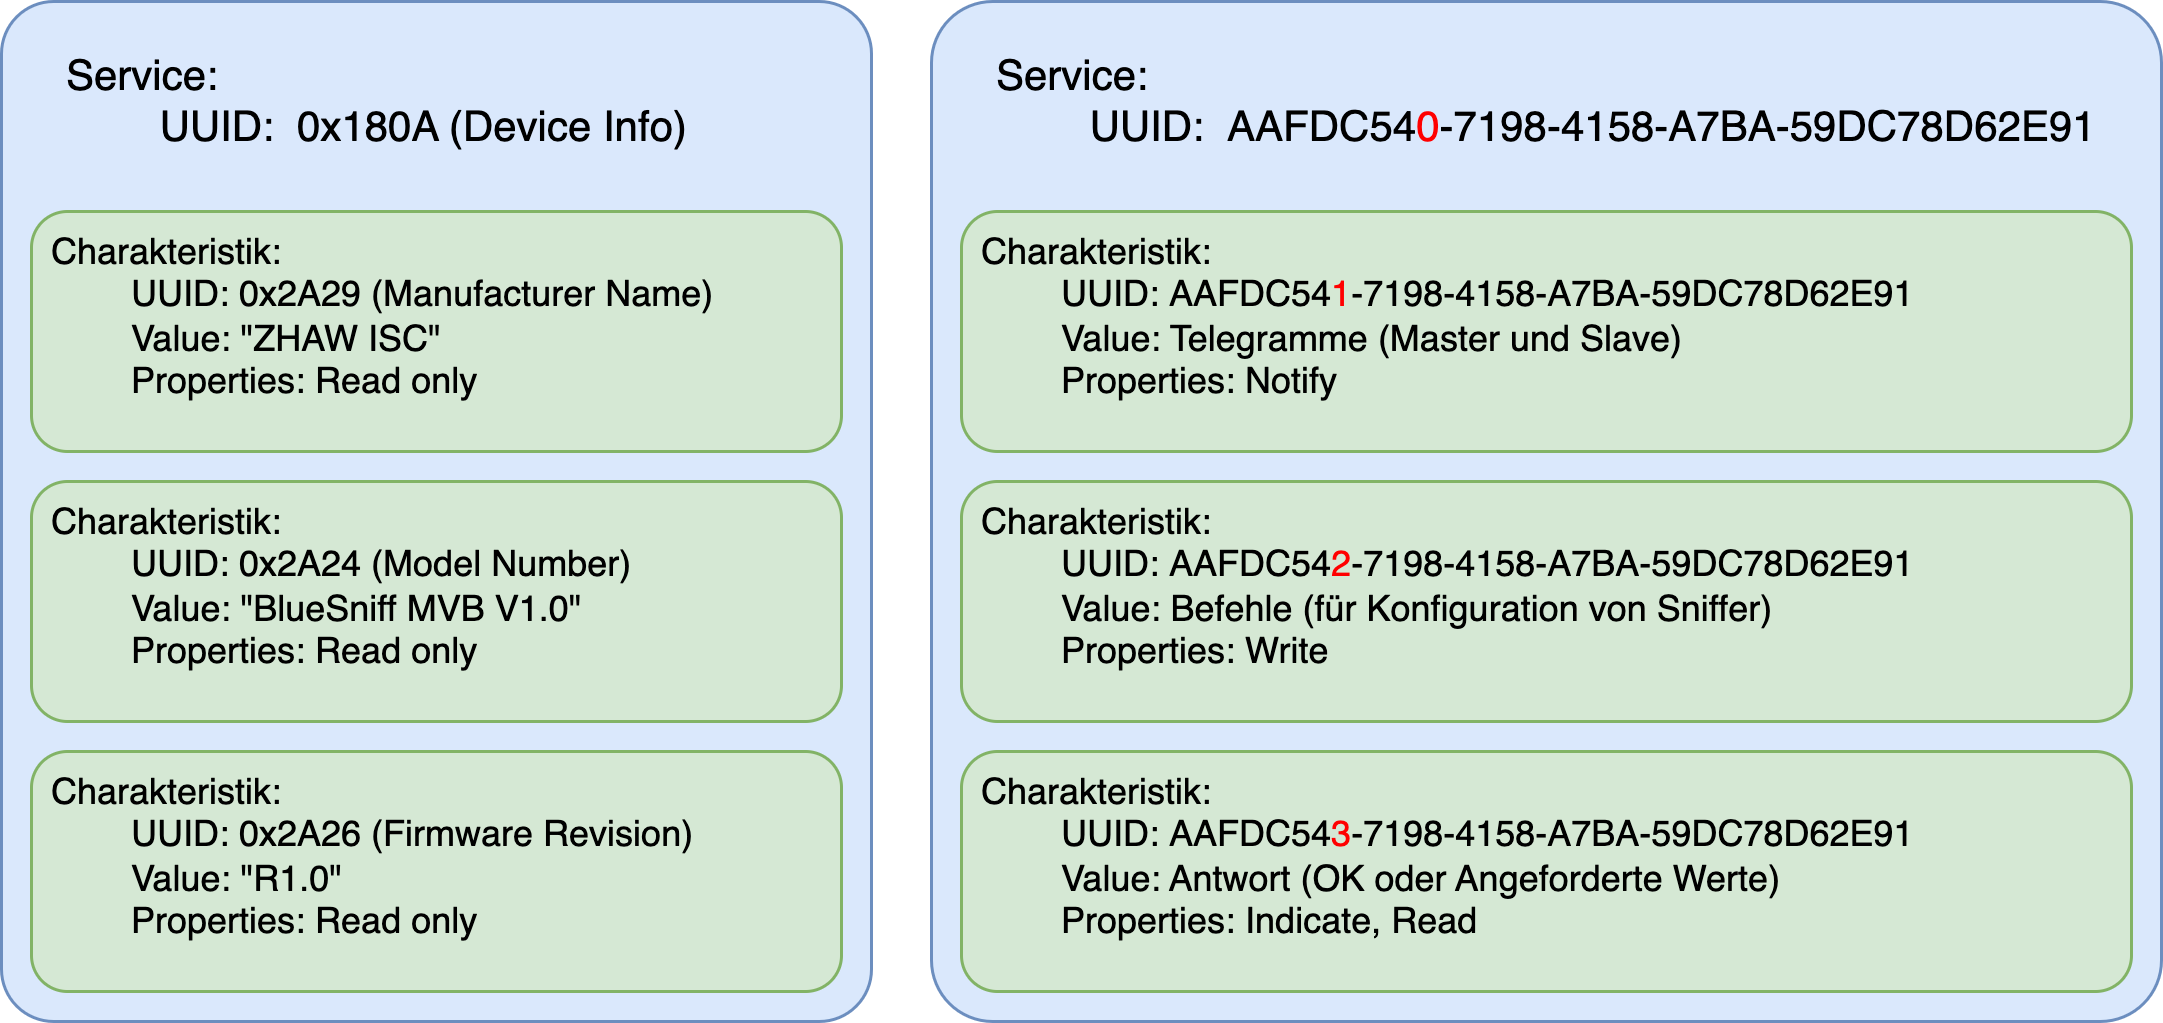
\includegraphics[width=0.9\linewidth]{Figures/Chap3/ESP/BLE/BLE.png}
%     \caption{Bluetooth GATT Server auf ESP32S3}
%     \label{fig:BLEGATT}
% \end{figure}

% \subsubsection{Service - Device Info}
% Der Service \textit{0x180A} zur \textit{Device Info} stellt dabei grundlegend statische Werte zur Verfügung, welche die Identifikation des Gerätes mit \textit{0x2A24 Model Number}, oder die Aktualität der Firmware \textit{0x2A26 Firmware Revision} nach aussen zur Verfügung stellen.

% \subsubsection{Service - Sniffer}
% Der zweite Service stellt keine vordefinierte 16bit UUID zur Verfügung. Daher wurde diese Service-UUID mithilfe eines \textit{Online UUID Generator} generiert. In Abbildung \ref{fig:BLEGATT} ist die Zahl an 8. Stelle rot markiert. Dies soll darauf hinweisen, dass diese Zahl für die Charakteristiken inkrementiert wurde. Der selbstdefinierte Service soll den Datenaustausch zwischen Sniffer und Endgerät handeln. 

% Die Charakteristik mit der roten Zahl 1 soll dabei die empfangenen Telegramme nach aussen schicken. Der erwartete Data-Throughput ist gemäss Kapitel \ref{tab:Busauslastung} bei Übertragung des gesamten MVB-Traffics hoch. Aus diesem Grund ist die \textit{Propertie} dieser Charakteristik auf \textbf{Notify} gesetzt.

% Die Charakteristik mit der roten Zahl 2 soll ein individualisierbares Befehlsset schicken können, womit der Sniffer gesteuert, beziehungsweise dessen Verhalten geändert werden kann. Beispiele dazu sind Einstellung eines Filters oder Abfrage von Parametern (siehe dazu Kapitel \ref{sec:Ausblick}). Weil die Befehle auf den Sniffer geschrieben werden, ist die \textit{Propiertie} in diesem Fall \textbf{Write}.

% Die Charakteristik mit der roten Zahl 3 soll die Befehle, welche mit der vorherigen Charakteristik geschickt worden sind, mit einer OK-Message bestätigen oder einen Payload haben. Die \textit{Propiertie} ist auf \textbf{Indicate} gesetzt, sodass der Sniffer eine Rückmeldung schickt, sobald er diese bereit hat. Im Falle eines Timeouts kann das Endgerät auch einen \textbf{Read} auf die Charakteristik machen




% \newpage

% %----------------------------------------------------------------------
% % SECTION Hardware PCB
% %----------------------------------------------------------------------
% \section{Hardware PCB}

% In diesem Unterkapitel wird die Entwicklung der Hardware für den MVB-Sniffer beschrieben. Zu den Kernkomponenten zählen der RS485-Transceiver SP3485CN-L/TR, das FPGA 10M08SAE144C8G und der Mikrocontroller ESP32-S3-WROOM-1. Die Hauptaufgabe besteht darin, die Funktionalitäten der drei Evaluationsboards zu analysieren und die Bauteile auf die für die Anwendung als MVB-Sniffer notwendigen Komponenten zu reduzieren. Dabei wurde auch berücksichtigt, welche zusätzlichen Funktionen in der weiteren Entwicklung von Nutzen sein könnten. Ziel ist ein für den Anwendungszweck optimiertes PCB-Design zu erstellen, das alle wesentlichen Anforderungen für die Signalverarbeitung und -analyse erfüllt und die verschiedenen elektronischen Bauteile und Module in einem kompakten Design vereint. Im Rahmen dieser Arbeit wurde zunächst ein Schema erstellt, welches als Grundlage für die spätere Entwicklung des PCBs dient. Als Software wurde hierfür Altium verwendet. Nachfolgend werden die zentralen Funktionen anhand der Schemata erläutert.


% \subsection{RS485-Transceiver}

% Das MVB-Signal wird durch den Sniffer über die beiden D-Sub-Stecker J1 und J2 durchgeführt und abgegriffen. Anschliessend wird es zum RS485-Transceiver weitergeleitet, wie in Abbildung \ref{fig:MVB to RS485} dargestellt. Der RS485-Transceiver verarbeitet die differentiellen Signale des MVB \textit{Data P} und \textit{Data N}. Er wandelt diese in ein einheitliches Signal \textit{MVB Data} um, das für die Weiterverarbeitung durch den FPGA verwendet wird. Dabei wird lediglich die 3 Leitungen der Linie A des MVB-Signals analysiert, während die redundante Linie B nicht abgegriffen wird, da sie in Fahrzeugen in der Praxis selten verwendet wird.

% Zur Stabilisierung der Versorgungsspannung \textit{Vcc 3V3} wird ein Stützkondensator eingesetzt, der nahe am Transceiver positioniert ist, um Spannungsschwankungen und Rauschen zu minimieren. 
% \textcolor{red}{Bild aktualisieren}
% \begin{figure}[H]
%     \centering
%     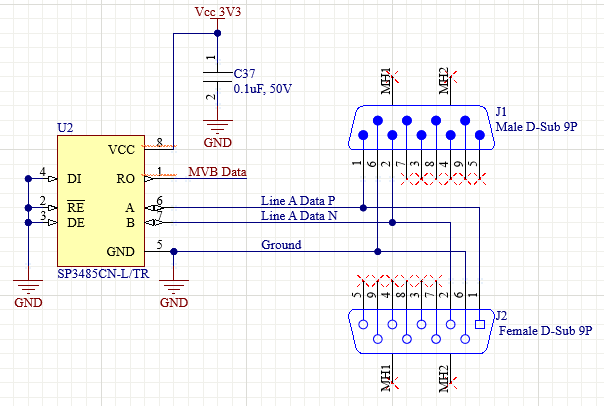
\includegraphics[width=0.8\linewidth]{Figures/Chap3/Schematics/MVB to RS485.png}
%     \caption{Vom MVB Signal zum RS485}
%     \label{fig:MVB to RS485}
% \end{figure}


% \subsection{FPGA}
% Ein FPGA ist ein flexibler Chip, der aus programmierbaren Logikblöcken, I/O-Banken und Verbindungsnetzwerken besteht. Die Konfiguration entscheidet, welche Funktionen der FPGA übernimmt und wie die einzelnen Blöcke und Schnittstellen zusammenarbeiten. Der 10M08SAE144C8G verfügt über 8 Banken, die unterschiedlich konfiguriert werden können. Für die Anwendung im MVB-Sniffer, wurde nur die Hälfte der Banken verwendet jedoch alle 8 Bänke mit Spannung versorgt, um für die Weiterentwicklung flexibel zu sein und um Störungen oder unerwartetes Verhalten zu vermeiden.


% \subsubsection{Programmierung}

% Programmiert wird der FPGA über die JTAG-Schnittstelle (Joint Test Action Group) ist ein standardisiertes Protokoll zur Programmierung, Konfiguration und Debugging von elektronischen Bausteinen wie Mikrocontrollern oder FPGA. Über die JTAG-Signale \textit{TCK} (Test Clock), \textit{TMS} (Test Mode Select), \textit{TDI} (Test Data Input) und \textit{TDO} (Test Data Output) können Daten seriell übertragen werden. Das Signal \textit{JTAGEN} (JTAG Enable) aktiviert die JTAG-Funktion. Im FPGA wird die Bank 1B für die JTAG-Schnittstelle verwendet, die eine zentrale Rolle bei der Konfiguration des FPGA spielt. Dies konnte vom Evaluationsboard übernommen werden, da auch dieses so programmiert wird. Es sind zwei Modi möglich:

% \begin{enumerate}
%     \item Direkte Konfiguration über .sof-Dateien:
%     Mithilfe des JTAG-Steckers kann eine .sof-Datei direkt in das FPGA geladen werden. Diese Datei enthält die Informationen für die momentane Programmierung des FPGAs. Dabei wird der FPGA bei einem Neustart oder einer erneuten Konfiguration in einen leeren Zustand versetzt, da die Konfiguration nur temporär gespeichert wird.
%     \item Programmierung der Configuration Flash Memory (CFM) mit .pof-Dateien: 
%     Alternativ kann über den JTAG-Header eine .pof-Datei in das CFM des FPGA programmiert werden. In diesem Fall startet der FPGA nach jedem Neustart automatisch in den Selbstkonfigurationsmodus und lädt die gespeicherten Daten aus dem CFM.
% \end{enumerate}

% \begin{figure}[H]
%     \centering
%     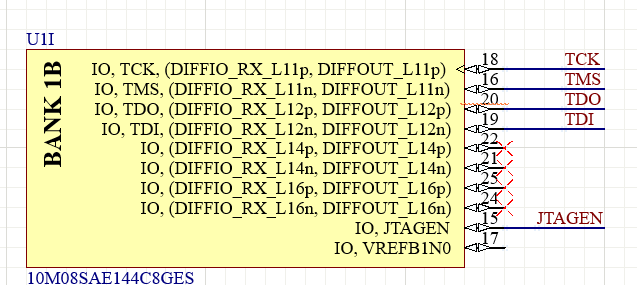
\includegraphics[width=0.5\linewidth]{Figures/Chap3/Schematics/Bank1B_JTAG.png}
%     \caption{FPGA Bank 1B: JTAG}
%     \label{FPGA JTAG}
% \end{figure}
% \textcolor{red}{Bilder aktualisieren}

% Wie in Abbildung \ref{FPGA JTAG} ersichtlich ist die JTAG Schnittstelle der Stecker \textit{J6}, welche mit einem USB-Blaster verbunden werden kann. Die 10 kOhm Widerstände sorgen dafür, dass die Signale \textit{TCK}, \textit{TMS}, und \textit{JTAGEN} auf logisch \textit{"1"} gehalten werden, wenn sie nicht aktiv angesteuert werden. Dies verhindert Fehlfunktionen durch unbestimmte Pegel. Der 1 kOhm Widerstand hält \textit{TDI} auf logisch \textit{"0"}, wenn kein Signal anliegt, auch um ungewollte Signalpegel zu vermeiden. Somit werden die Signale über die Pins des Steckers \textit{J6} mit dem FPGA verbunden, \textit{JTAGEN} wird auf logisch \textit{"1"} gezogen, wodurch das FPGA in den Programmierungsmodus versetzt wird und über die restlichen Pins die Programmdaten und Steuersignale an das FPGA sendet.


% \subsubsection{Oszillator}

% Es wird analog zum Evalutionsboard der Oszillator CB3LV-3C-50M0000 verwendet, um einen stabilen und präzisen externen Takt von 50 MHz bereitzustellen. Dieser Takt wird benötigt um die Abläufe im FPGA zu synchronisieren und zusätzliche Takte zu erzeugen, die es für bestimmte Aufgaben braucht. Dafür wird der Oszillator mit einem dedizierten Clock-Pin des FPGA verbunden auf der Bank 2 (siehe Abbildung \ref{FPGA OSC}).
% \begin{figure}[H]
%     \centering
%     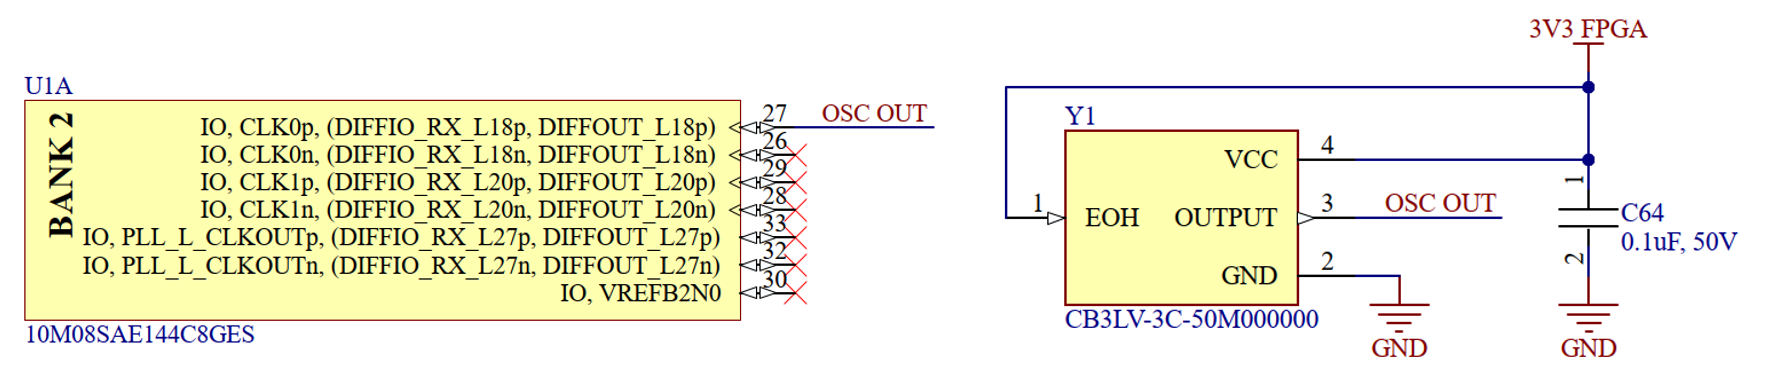
\includegraphics[width=0.6\linewidth]{Figures/Chap3/Schematics/Bank2_OSC.png}
%     \caption{FPGA Bank 2: Oscillaror}
%     \label{FPGA OSC}
% \end{figure}
% \textcolor{red}{Bilder aktualisieren}


% \subsubsection{Steuersignale}

% Auf der Bank 8 des FPGA gibt es mehrere Steuersignale, die in der zukünftigen Anwendung von wichtger Bedeutung sein können.

% \begin{itemize}
%     \item Durch das Betätigen des Knopfes S4 wird das FPGA gezwungen, sich aus dem Configuration Flash Memory (CFM) neu zu konfigurieren. Dieser Knopf ist mit Pin 129 des FPGA verbunden mit dem Signal \textit{NCONFIG}. Da in Zukunft Programmierung über die CFM laufen soll erscheint diese Funktion als wichtig.
    
%     \item Das Betätigen des Knopfes S4 setzt alle Register im FPGA zurück. Dies kann für eine schnelle Rücksetzung des Systems genutzt werden, ohne das FPGA vollständig neu zu konfigurieren. Das Signal \textit{RESET N} wird auf den dafür vorgesehenen Pin 121 geführt.
    
%     \item Mit diesem Schalter SW1 wird ausgewählt, welches CFM-Bild (Konfigurationsbild) beim Start des FPGA verwendet wird, wenn eine Dual-Image-Konfiguration vorliegt. Diese Funktionen ermöglichen eine flexible Konfiguration und Steuerung des FPGA, insbesondere wenn in einem zukünftigen Schritt mehrere Konfigurationsoptionen gefordert werden, wie zum Beispiel eine Umschaltung von ESD auf EMD.
% \end{itemize}

% \begin{figure}[H]
%     \centering
%     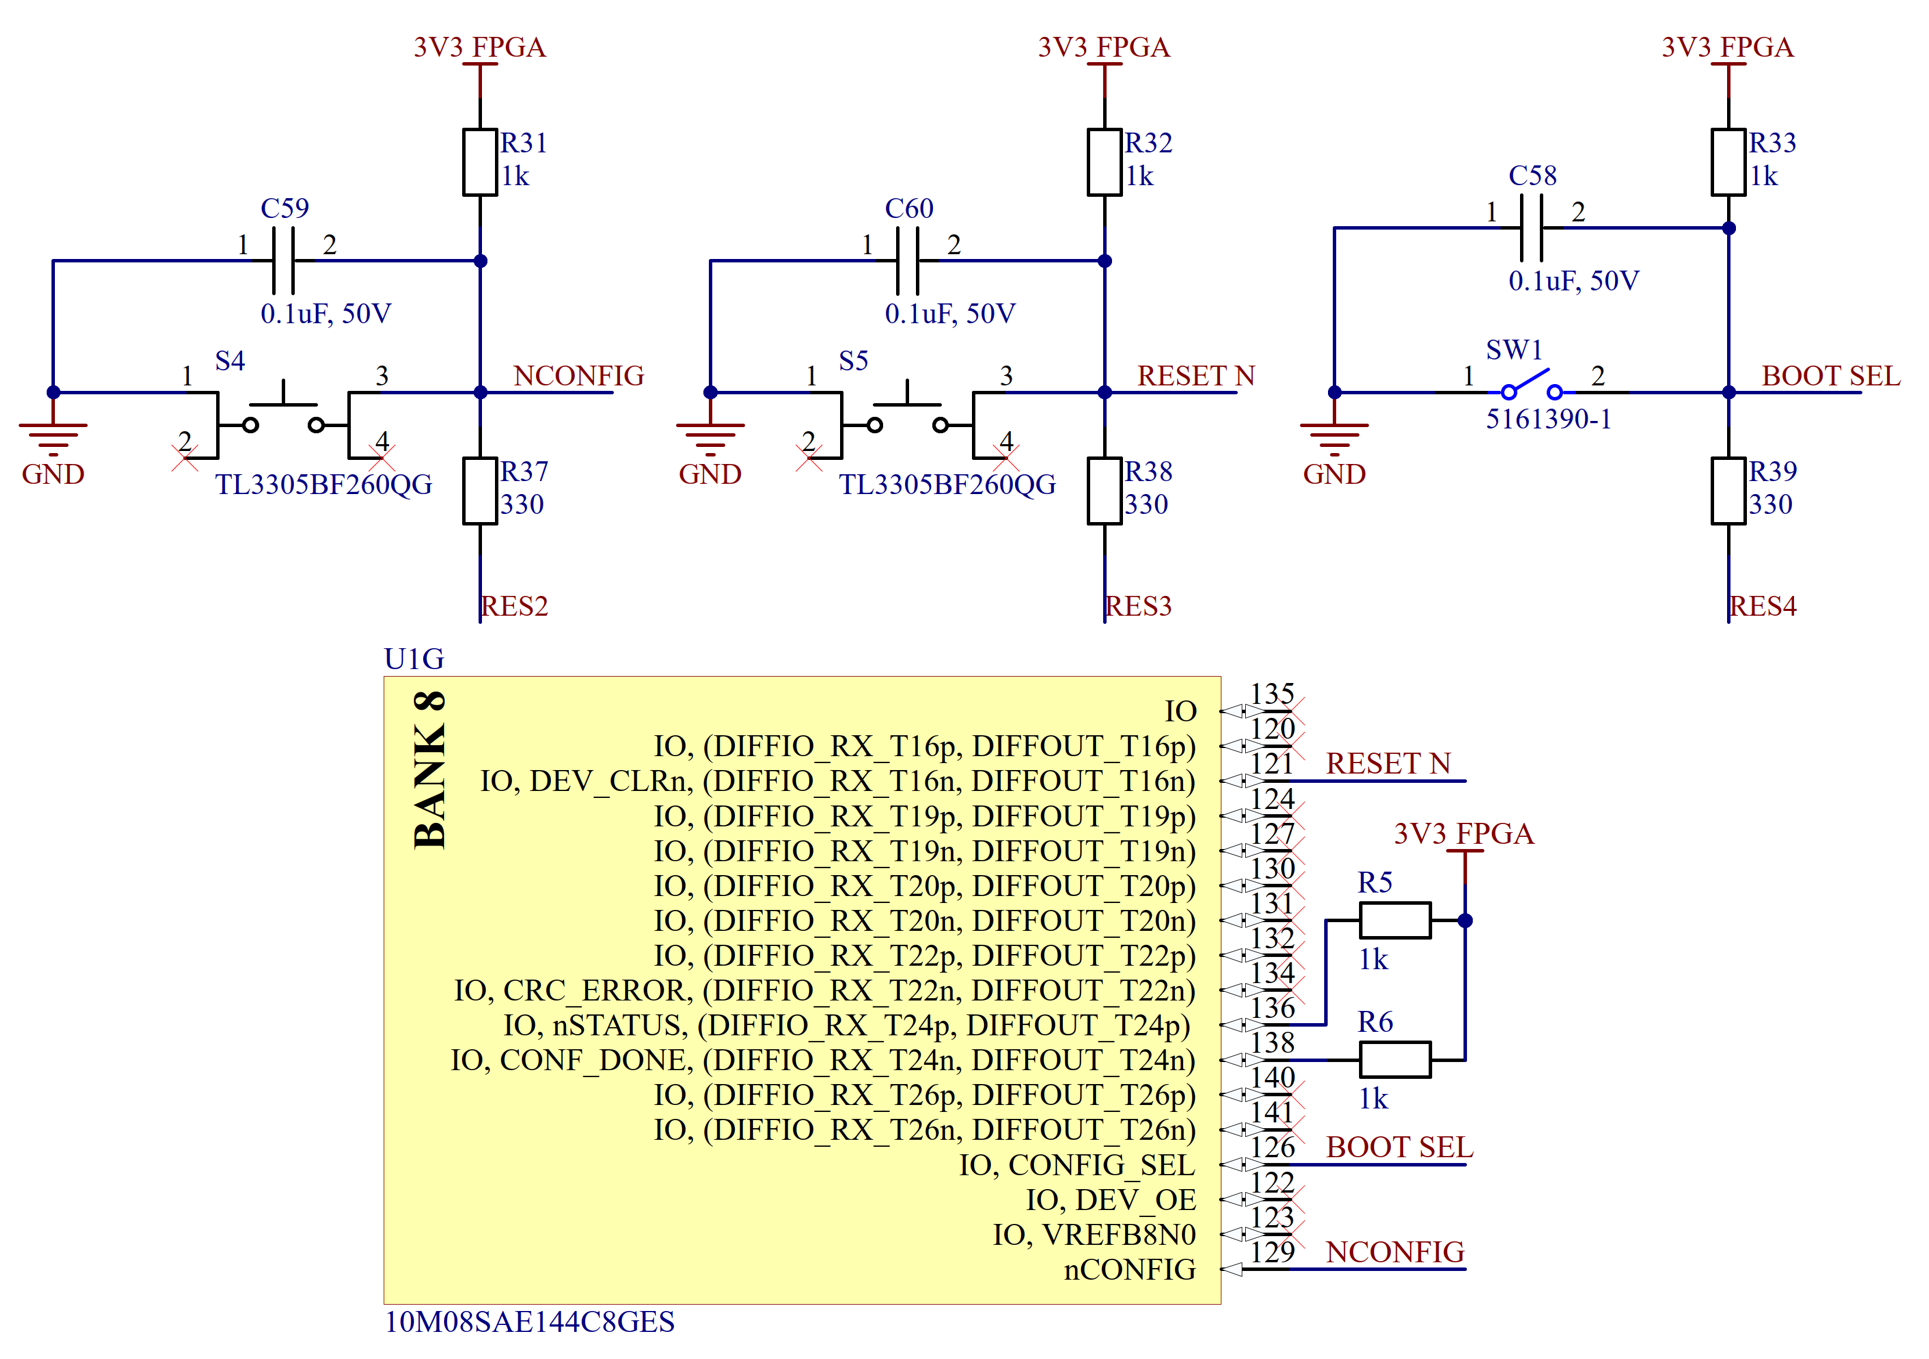
\includegraphics[width=0.8\linewidth]{Figures/Chap3/Schematics/Bank8_Admin.png}
%     \caption{FPGA Bank 8: Konfiguration}
%     \label{FPGA Admin}
% \end{figure}
% \textcolor{red}{Bilder aktualisieren}


% \subsubsection{ESP32-S3 Schnittstellen}

% Für die Kommunikation zwischen dem FPGA, dem ESP32 und dem RS485 wurde Bank 3 vorgesehen. In dieser Bank sind die SPI-Signale (\textit{CS, MOSI, MISO} und \textit{SCLK}) so verbunden, dass eine direkte Kommunikation zwischen dem FPGA und dem ESP32 ermöglicht wird. Zusätzlich wurde eine Handshake-Leitung \textit{HS FPGA} und Interrupt-Leitungen \textit{INTR FPGA} integriert, um künftige Erweiterungen zu unterstützen.

% Darüber hinaus stehen die Reserveleitungen \textit{RES1} bis \textit{RES4} zur Verfügung. Diese Leitungen haben derzeit noch keine festgelegte Funktion, sind jedoch ebenfalls als Verbindungen zwischen FPGA und ESP32 vorgesehen.

% Für das Signal \textit{MVB Active} wurde eine LED-Ansteuerung mithilfe eines Darlington-Arrays vorgesehen (Details dazu weiter unten in Kapitel \ref{ESP32-S3}).

% Zusätzlich wurde ein \textit{IO RES FPGA} Pin über einen Steckverbinder ausgeführt, um bei zukünftigen Weiterentwicklungen flexibel und schnell reagieren zu können.

% \begin{figure}[H]
%     \centering
%     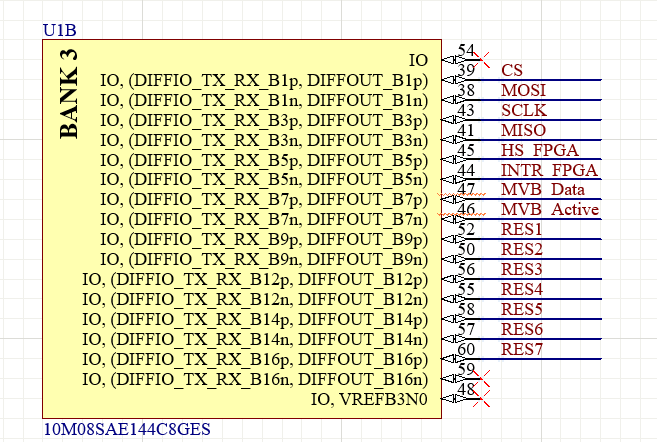
\includegraphics[width=0.6\linewidth]{Figures/Chap3/Schematics/Bank3_ESP.png}
%     \caption{FPGA Bank 3: ESP32 Interface}
%     \label{FPGA ESP}
% \end{figure}
% \textcolor{red}{Bilder aktualisieren}

% \subsubsection{Peripherie FPGA}


% \subsection{ESP32-S3}
% \textcolor{red}{Wie wurde der ESP auf der Platine integriert}


% \subsubsection{USB UART}


% \subsubsection{USB-A}


% \subsubsection{Peripherie ESP32-S3}


% \subsection{Indikatoren}

